\documentclass[a4paper, 14pt]{report}

\setcounter{secnumdepth}{3}
\setcounter{tocdepth}{3}


\usepackage[vietnamese=nohyphenation]{hyphsubst}
\usepackage[english, vietnamese]{babel}
\usepackage{indentfirst} % indent first paragraph
\usepackage{geometry} % set page margin

\usepackage{tikz} %vẽ bìa

\usepackage{enumerate}
\usepackage{amsmath}
% \usepackage{amsfonts}
\usepackage{amssymb}
\usepackage{color}



\usepackage{url}

\usepackage{pgfplots}



\usepackage{amsthm}
\usepackage[unicode]{hyperref}

\usepackage{fontspec}
\usepackage{graphicx}
\usepackage{enumitem}
\usepackage{a4wide}
\usepackage{epsfig}
\usepackage{latexsym}
\usepackage{array}
\usepackage{hhline}

\usepackage[normalem]{ulem}
\usepackage[makeroom]{cancel}
\usepackage{longtable}
\usepackage{amscd}
\usepackage{diagbox}
\usepackage{booktabs}
\usepackage{alltt}
\usepackage[framemethod=tikz]{mdframed}
\usepackage{subcaption}
\usepackage{caption}
\usepackage{listings}
\usepackage{xcolor}
\usepackage{lipsum}
\usepackage{setspace}

\usepackage{multicol}
\usepackage{indentfirst}
\usepackage{float}
\usepackage{titlesec}
\usepackage[nottoc]{tocbibind}
\usepackage[autostyle]{csquotes}

\urlstyle{rm}

\usetikzlibrary{decorations}
\usetikzlibrary{decorations.pathreplacing}
\usetikzlibrary{decorations.pathreplacing,calligraphy}
\usetikzlibrary{arrows.meta}
\usetikzlibrary{quotes}

\usetikzlibrary{intersections}
\usetikzlibrary{calc}
\usetikzlibrary{arrows}

\setstretch{1.3}

\usepackage{caption}

\captionsetup{
font=Large
}

\pgfplotsset{compat=1.15}

\setlength{\baselineskip}{6pt}

\theoremstyle{definition}


\renewcommand\thechapter{\Roman{chapter}}
\renewcommand\thesection{\arabic{section}}
\renewcommand\thesubsection{\thesection.\arabic{subsection}}
\renewcommand*{\thesubsubsection}{\thesubsection.\arabic{subsubsection}}

\newtheorem{theorem}{Định lý}[section]
\newtheorem{acknowledgement}[theorem]{Acknowledgement}
\newtheorem{algorithm}[theorem]{Algorithm}
\newtheorem{axiom}[theorem]{Axiom}
\newtheorem{case}[theorem]{Case}
\newtheorem{claim}[theorem]{Claim}
\newtheorem{conclusion}[theorem]{Conclusion}
\newtheorem{condition}[theorem]{Condition}
\newtheorem{conjecture}[theorem]{Conjecture}
\newtheorem{corollary}[theorem]{Corollary}
\newtheorem{criterion}[theorem]{Criterion}
\newtheorem{definition}{Định nghĩa}
\newtheorem{example}{Ví dụ}
\newtheorem{exercise}[theorem]{Exercise}
\newtheorem{lemma}[theorem]{Lemma}
\newtheorem{notation}[theorem]{Notation}
\newtheorem{problem}[theorem]{Problem}
\newtheorem{proposition}[theorem]{Mệnh đề }
\newtheorem{remark}{Nhận xét}
\newtheorem{solution}[theorem]{Solution}
\newtheorem{summary}[theorem]{Summary}

\geometry{
    top=2.5cm,
    bottom=3cm,
    left=3.5cm,
    right=2cm
}

\setmainfont{Times New Roman}
\titleformat{\section}
  {\bfseries\fontsize{18}{20}\selectfont\rmfamily}{\thesection}{1em}{}
\titleformat{\subsection}
  {\bfseries\fontsize{16}{18}\selectfont\rmfamily}{\thesubsection}{1em}{}
\titleformat{\subsubsection}
  {\bfseries\fontsize{14}{16}\selectfont\rmfamily}{\thesubsubsection}{1em}{}

\definecolor{dkgreen}{rgb}{0,0.6,0}
\definecolor{gray}{rgb}{0.5,0.5,0.5}
\definecolor{mauve}{rgb}{0.58,0,0.82}
\everymath={\displaystyle}
\newmdenv[linecolor=gray,skipabove=\topsep,skipbelow=\topsep,
leftmargin=-5pt,rightmargin=-5pt,
innerleftmargin=5pt,innerrightmargin=5pt]{mybox}

\lstset{
  % frame=tb,
  language=Python,
  aboveskip=3mm,
  belowskip=3mm,
  showstringspaces=false,
  columns=flexible,
  basicstyle={\small\ttfamily},
  numbers=left,
  numberstyle=\tiny\color{gray},
  keywordstyle=\color{blue},
  commentstyle=\color{dkgreen},
  stringstyle=\color{mauve},
  breaklines=true,
  breakatwhitespace=true,
  tabsize=4
}



\title{Blockchain trong truy xuất nguồn gốc thực phẩm}

\author{
{
    Lê Thị Thùy Dung\thanks{Khoa Toán-Cơ-Tin học, Đại học Khoa học Tự Nhiên, }}
}
\date{}


\begin{document}
\pagestyle{empty}
\begin{titlepage}
    \thispagestyle{empty}
    \begin{tikzpicture}[overlay,remember picture]
    \draw [line width=2pt]
        ($ (current page.north west) + (3.5cm,-2.5cm) $)
        rectangle
        ($ (current page.south east) + (-2cm,2.5cm) $);
        \draw [line width=0.5pt]
    ($ (current page.north west) + (3.6cm,-2.6cm) $)
    rectangle
    ($ (current page.south east) + (-2.1cm,2.6cm) $); 
    \end{tikzpicture}
    \begin{center}        
        {\fontsize{14}{10}\selectfont 
        ĐẠI HỌC QUỐC GIA HÀ NỘI\\
        ĐẠI HỌC KHOA HỌC TỰ NHIÊN\\
        \fontsize{13}{16}\selectfont \textbf{KHOA TOÁN - CƠ - TIN HỌC}
        }
        \end{center}
        
        \vspace*{3cm}
        
        \begin{center}
            {
    
                \fontsize{14}{0}\selectfont \textbf{LÊ THỊ THÙY DUNG}
            }
        \end{center}
        \begin{center}
       
        \vspace*{3cm}
        { 
            \fontsize{18}{24}\selectfont \textbf{ BLOLCKCHAIN TRONG TRUY XUẤT NGUỒN \\ GỐC THỰC PHẨM}}
        \end{center}
        \vspace*{2cm}
        \begin{center}
        {
        \fontsize{14}{16}\selectfont Khóa luận tốt nghiệp dành cho đại học chính quy \\
        \fontsize{14}{16}\selectfont Ngành Máy tính và Khoa học Thông tin \\
        (Chương trình đào tạo chuẩn)
        }
        \end{center}
        %  \centerline{\Huge\bf PHƯƠNG PHÁP GIẢI TOÁN }
        % \vspace*{0.5cm}
        
        \vfill
         \centerline{
            \fontsize{14}{0}\selectfont \textbf{ HÀ NỘI - 2023}}
        
    \end{titlepage}
    
    
\begin{titlepage}
    \begin{tikzpicture}[overlay,remember picture]
    \draw [line width=2pt]
        ($ (current page.north west) + (3.5cm,-2.5cm) $)
        rectangle
        ($ (current page.south east) + (-2cm,2.5cm) $);
        \draw [line width=0.5pt]
    ($ (current page.north west) + (3.6cm,-2.6cm) $)
    rectangle
    ($ (current page.south east) + (-2.1cm,2.6cm) $); 
    \end{tikzpicture}
    \begin{center}        
        {\fontsize{14}{10}\selectfont 
        ĐẠI HỌC QUỐC GIA HÀ NỘI\\
        ĐẠI HỌC KHOA HỌC TỰ NHIÊN\\
        \fontsize{13}{16}\selectfont \textbf{KHOA TOÁN - CƠ - TIN HỌC}
        }
        \end{center}
        
        \vspace*{3cm}
        
        \begin{center}
            {
                \fontsize{14}{0}\selectfont \textbf{LÊ THỊ THÙY DUNG}
            }
        \end{center}
        \begin{center}
       
        \vspace*{3cm}
        {\fontsize{18}{24}\selectfont \textbf{ BLOLCKCHAIN TRONG TRUY XUẤT NGUỒN \\ GỐC THỰC PHẨM}}
        \end{center}
        \vspace*{2cm}
        \begin{center}
        {
        \fontsize{14}{16}\selectfont Khóa luận tốt nghiệp dành cho đại học chính quy \\
        \fontsize{14}{16}\selectfont Ngành Máy tính và Khoa học Thông tin \\
        (Chương trình đào tạo chuẩn)
        }
        \end{center}
  
        \vspace*{1cm}
        \begin{center}
            {
                \fontsize{14}{0}\selectfont \textbf{ Cán bộ hướng dẫn: PGS.TS. PHÓ ĐỨC TÀI}
            }
        \end{center}
        \vfill
         \centerline{
            \fontsize{14}{0}\selectfont \textbf{ HÀ NỘI - 2023}}
        
    \end{titlepage}
    
    
\chapter*{Lời cảm ơn}
\thispagestyle{empty}
\fontsize{14}{16}\selectfont
\begin{center}
\end{center}
\hspace*{1.5cm}Đầu tiên em xin gửi lời cảm ơn đặc biệt và sâu sắc tới PGS.TS. Phó Đức Tài, Trưởng
khoa Toán – Cơ – Tin học, thầy đã trực tiếp hướng dẫn đề tài khoá luận này của em.
Thầy đã cho em ý tưởng và giúp đỡ em tận tình trong suốt quá trình thực hiện đề tài. \\
\hspace*{1.5cm} Em xin chân thành cảm ơn các thầy cô công tác tại khoa Toán – Cơ – Tin học,
Trường Đại học Khoa học Tự nhiên, Đại học Quốc gia Hà Nội. Trong quá trình bốn
năm học tập và rèn luyện tại khoa, em đã được các thầy cô hết lòng chỉ bảo và tạo
điều kiện để em có thể hoàn thành tốt cả việc học tập và các nhiệm vụ được giao
khác.

Và cuối cùng, tôi xin cảm ơn tới bạn bè, đặc biệt là gia đình và người thân luôn 
ủng hộ, động viên tôi trong suốt quá trình thực hiện khoá văn. Mặc dù đã cố gắng hết sức, tuy 
nhiên trong quá trình thực hiện em không tránh khỏi được những thiếu sót, em rất mong nhận được 
sự thông cảm và đánh giá chân tình của bạn bè và thầy cô để khoá văn của em được hoàn thiện hơn nữa.
\begin{flushright}
{\it Hà Nội, ngày ... tháng ... năm 2023}

Sinh viên\hskip 2cm\quad

\vskip 1cm
{\bf Lê Thị Thuỳ Dung} \hskip 1cm \quad\ 
 \end{flushright}



\newpage
\section*{Danh mục các ký hiệu và chữ viết tắt}
\thispagestyle{empty}

\begin{table}[htbp]
  \fontsize{14}{16}\selectfont
    \begin{center}
      \begin{tabular*}{\linewidth}{@{\extracolsep{\fill}}|>{\centering}m{0.1\linewidth}|>{\centering\arraybackslash}m{0.2\linewidth}|>{\centering\arraybackslash}m{0.25\linewidth}|>{\centering\arraybackslash}m{0.25\linewidth}|}
        \hline
        \textbf{STT} & \textbf{Chữ viết tắt} & \textbf{Diễn giải} & \textbf{Tiếng Việt} \\
        \hline
        01 & SHA & Secure Hash Algorithm & Thuật toán băm an toàn  \\
        \hline
        02 & ECDSA & Elliptic Curve Digital Signature Algorithm & Chữ ký số trên đường cong elliptic \\
        \hline
        03 & ECC & Elliptic Curve Cryptography & Mật mã đường cong elliptic \\
        \hline
        04 & PoW & Proof of work & Bằng chứng công việc \\
        \hline
        05 & PoS & Proof of stake & Bằng chứng cổ phần \\
        \hline
        06 & CA & Certificate Authorities & Tổ chức phát hành chứng chỉ \\
        \hline
        07 & MSB & Member Service Provider & Nhà cung cấp dịch vụ thành viên \\
        \hline
      \end{tabular*}
    \end{center}
  \end{table}
  


\tableofcontents

\newpage
\pagestyle{plain}

\chapter*{Mở đầu}
\setcounter{page}{1}
Truy xuất nguồn gốc thực phẩm là quá trình xác định nguồn gốc và lịch sử sản xuất của một sản phẩm
thực phẩm từ giai đoạn sản xuất đến khi đến tay người tiêu dùng. Ý nghĩa của việc truy xuất nguồn 
gốc thực phẩm là giúp người tiêu dùng đảm bảo được an toàn về chất lượng và nguồn gốc của sản phẩm
mà mình sử dụng, đồng thời cũng là một phương tiện quan trọng giúp kiểm soát và ngăn chặn sự xuất
hiện của những sản phẩm thực phẩm giả mạo, không rõ nguồn gốc và an toàn.

Việc truy xuất nguồn gốc thực phẩm đang được xem là một xu hướng quan trọng trong ngành thực phẩm,
đặc biệt là trong bối cảnh ngày nay, khi mối đe dọa về an toàn thực phẩm và việc giả mạo sản phẩm 
thực phẩm ngày càng trở nên phức tạp. Việc thực hiện truy xuất nguồn gốc thực phẩm sẽ giúp tăng
cường niềm tin của người tiêu dùng đối với sản phẩm thực phẩm và giúp nâng cao chất lượng và an toàn thực phẩm trên thị trường.

Truy xuất nguồn gốc thực phẩm được thực hiện thông qua việc ghi nhận, lưu trữ và quản lý các thông
tin liên quan đến quá trình sản xuất và phân phối sản phẩm thực phẩm, bao gồm nguồn gốc, thời gian
sản xuất, địa điểm sản xuất, thông tin về các thành phần, chất lượng, độ an toàn của sản phẩm. 
Những thông tin này được ghi nhận và kiểm soát bởi các cơ quan chức năng, doanh nghiệp và các tổ 
chức liên quan trong quá trình sản xuất và phân phối sản phẩm.

Với sự phát triển của công nghệ Blockchain, việc áp dụng Blockchain để giải quyết việc truy xuất nguồn gốc 
thực phẩm trở nên khả quan hơn. Công nghệ Blockchain cho phép lưu trữ thông tin về nguồn gốc, vận chuyển và quản lý 
các sản phẩm thực phẩm một cách minh bạch, chính xác và an toàn.


Trong bài toán truy xuất nguồn gốc thực phẩm sử dụng công nghệ Blockchain, các thông tin về nguồn 
gốc, chất lượng và quá trình sản xuất của sản phẩm sẽ được lưu trữ trên một mạng lưới phi tập trung,
nơi mà các bên liên quan có thể truy cập và xác minh thông tin một cách dễ dàng. Điều này giúp cho 
người tiêu dùng có thể kiểm tra được nguồn gốc và chất lượng của sản phẩm mà mình mua, giảm thiểu 
nguy cơ mua phải sản phẩm giả, kém chất lượng hoặc không đảm bảo vệ sinh an toàn thực phẩm.

Ngoài ra, việc sử dụng công nghệ Blockchain trong bài toán truy xuất nguồn gốc thực phẩm cũng giúp
cho các nhà sản xuất và đại lý có thể quản lý sản phẩm một cách chính xác hơn, đảm bảo tính minh 
bạch và giảm thiểu chi phí trong quá trình quản lý hàng hóa. Từ đó, giúp cho ngành công nghiệp thực
phẩm phát triển bền vững và đáp ứng được nhu cầu của thị trường ngày càng khắt khe.

Em sẽ trình bày khóa luận này theo hướng đi từ các kiến thức bổ trợ rồi đến bài toán chính.
Chương I cung cấp lý thuyết và các kiến thức cần thiết cho bài toán chính đặt ra ở Chương II.
Chương II trình bày về nền tảng Hyperledger Fabric.
Chương III sẽ trình bày về bài toán truy xuất nguồn gốc và ứng dụng các kiến thức để mô tả ứng dụng thử nghiệm và hướng phát triển.
Do còn hạn chế về kiến thức nên bài khóa luận sẽ có một số phần chưa đạt kết quả như mong muốn. 
Sự nhận xét, đánh giá và đóng góp ý kiến từ hội đồng sẽ là động lực để em hoàn thiện để
đề tài tốt hơn.

\chapter{Giới thiệu về công nghệ Blockchain}
\section{Nền tảng lý thuyết}
\subsection{Hàm băm}
\subsubsection{Tổng quan về hàm băm}
Hàm băm là một thuật toán được sử dụng để biến đổi dữ liệu đầu vào thành một chuỗi ngắn hơn và đại diện
cho dữ liệu đó, được gọi là giá trị băm. Giá trị đầu vào của hàm băm là tuỳ ý nhưng đầu ra của hàm băm là một giá trị 
cố định sẵn, được gọi là độ dài băm. Độ dài băm có thể là 128, 256 hoặc 512 bit.
Giá trị băm là duy nhất cho mỗi dữ liệu đầu vào và không thể dễ dàng được tái tạo ngược lại dữ liệu gốc ban đầu. Điều này đảm bảo tính toàn vẹn và 
bảo mật của dữ liệu.

Hàm băm có các tính chất để đảm bảo tính toàn vẹn và bảo mật của dữ liệu:
\begin{itemize}
\item[-] Tính một chiều: Hàm băm là đơn chiều, nghĩa là không thể dễ dàng 
tái tạo ngược dữ liệu đầu vào từ giá trị băm.
\item[-] Tính kháng va chạm yếu: đảm bảo rằng việc tìm kiếm hai dữ liệu đầu vào khác nhau có cùng 
giá trị băm là rất khó khăn. Tính va chạm yếu đóng vai trò quan trọng trong việc đảm bảo tính toàn
vẹn của dữ liệu và tránh các cuộc tấn công nhằm thay đổi dữ liệu đầu vào. 
\item[-] Tính kháng va chạm mạnh:  Tính kháng va chạm mạnh đảm bảo rằng việc tìm kiếm một cặp dữ 
liệu đầu vào cho ra cùng một giá trị băm là rất khó khăn và tốn nhiều thời gian, dữ liệu tính toán.
Tính kháng va chạm mạnh đóng vai trò quan trọng trong việc tăng cường tính bảo mật của hàm băm và 
đảm bảo tính toàn vẹn của dữ liệu.
\item[] 
\end{itemize}

Hàm băm được sử dụng rộng rãi trong các ứng dụng bảo mật và xác thực. Ví dụ như trong việc lưu trữ
mật khẩu của người dùng. Thay vì lưu trữ mật khẩu người dùng dưới dạng văn bản thông thường, hàm 
băm sẽ được sử dụng để biến đổi mật khẩu thành một giá trị băm duy nhất. Khi người dùng đăng nhập, 
hệ thống sẽ so sánh giá trị băm của mật khẩu được nhập vào với giá trị băm đã được lưu trữ. Nếu hai 
giá trị này khớp nhau, người dùng sẽ được cho phép truy cập vào hệ thống.

Hàm băm cũng được sử dụng trong việc xác minh tính toàn vẹn của dữ liệu trong quá trình truyền tải, 
nơi một giá trị băm được tạo ra cho dữ liệu và gửi đi cùng với dữ liệu ban đầu. Người nhận có thể 
sử dụng hàm băm để kiểm tra tính toàn vẹn của dữ liệu bằng cách so sánh giá trị băm nhận được với 
giá trị băm được gửi đi ban đầu. Nếu hai giá trị băm này khớp nhau, dữ liệu được xác định là chưa 
bị thay đổi trong quá trình truyền tải.

Một số hàm được sử dụng phổ biến trong các ứng dụng bảo mật và xác thực: MD5, SHA-1, SHA-256, SHA-512...
Trong đó SHA-256 được sử dụng phổ biến nhất vì tính toán nhanh, mức độ bảo mật cao.
\subsubsection{Hàm băm SHA-256}
Thuật toán Secure Hash Algorithm (SHA) được phát triển bởi Cơ quan An ninh
Quốc gia Hoa Kỳ (National Security Agency - NSA), để chuyển đổi độ dài dữ liệu thành một độ dài cố định.

SHA-256 là hàm băm có đầu ra có độ dài 256 bit. SHA-256 với kết quả đầu ra tương đương với $2^{256}$ bits.
Đây là một hàm băm an toàn bởi vì nó có độ khó tìm kiếm kháng va chạm mạnh. 

Có một số phương pháp để tấn công SHA-256 như :
\begin{itemize}
\item[-] Brute force: Đây là phương pháp tấn công đơn giản nhất, trong đó kẻ tấn công
thử tất cả các khóa để tìm ra giá trị băm phù hợp. 
\item[-] Tấn công preimage: Đây là phương pháp tìm kiếm đầu vào phù hợp với một giá 
trị băm đã biết trước. Nếu kẻ tấn công có thể tìm ra đầu vào phù hợp với giá trị băm, thì an toàn của hàm băm sẽ bị đe dọa.
\item[-] Tấn công collision: Đây là phương pháp tìm kiếm hai đầu vào khác nhau nhưng cho
cùng một giá trị băm. Nếu kẻ tấn công có thể tìm ra hai đầu vào như vậy, thì an toàn của hàm băm sẽ bị đe dọa.
\end{itemize}

Tấn công Brute-force khó thực hiện bởi vì độ dài của đầu vào là $2^{256}$ bits.
Hiện tại, Frontier xây dựng vào năm 2022 bởi công ty công nghệ thông tin đa quốc gia
Hewlett Packard Enterprise là siêu máy tính có tốc độ tính toán nhanh nhất hiện nay. Nó có thể tính
toán khoảng $10^{12}$ phép tính trên giây. Thế giới có 8 tỷ người, giả sử mọi người đều tính toán
không ngừng nghỉ, 1 năm sẽ tính được $2,52 \times 10^{32}$ phép tính. Vậy cần khoảng $1,23 \times 10^{40}$ năm để tính hết các 
trường hợp đầu ra của SHA-256. 

Tấn công collision và tấn công preimage cũng khó thực hiện bởi vì:
\begin{itemize}
    \item[-] Đầu vào có độ dài lớn: có thể lên tới $2^{256}$ bits.
    \item[-] Không thể tái tạo đầu vào từ giá trị băm: Với thuật toán băm như SHA-256, 
    việc tìm kiếm một đầu vào có cùng giá trị hash với một giá trị hash đã biết (tấn công preimage) cũng rất khó khăn. Điều này là do giá trị hash được tạo ra bằng cách áp dụng một hàm băm không thể đảo ngược (one-way function), tức là không thể tái tạo đầu vào ban đầu từ giá trị hash.
\end{itemize}

Bởi vậy SHA-256 là một hàm băm an toàn, được sử dụng phổ biến trong các ứng dụng bảo mật và xác thực.

\subsubsection{Các thức hoạt động SHA-256}
SHA-256 bao gồm các bước sau:

\begin{itemize}
    \item[\textbf{Bước 1: }] Khởi tạo giá trị đầu vào cho hàm băm SHA-256.
        \item[1.1:] Chuyển dữ liệu đầu vào thành chuỗi nhị phân.
        \item[1.2:] Thêm 1 bit 1 vào cuối chuỗi nhị phân.
        \item[1.3:] Nối 0 cho đến khi độ dài $l$ của chuỗi nhị phân thoả mãn $ l \mod 512 = 64$.
        \item[1.4:] Độ dài của dữ liệu đầu vào được chuyển thành chuỗi nhị phân 64 bits, 
        sau đó được thêm vào cuối chuỗi nhị phân. 
    \item[\textbf{Bước 2:}] Khởi tạo bộ đệm. \\
        Tạo các giá trị băm từ $H_1$ đến $H_8$ là 32 bit đầu tiên của
        căn bậc hai của 8 số nguyên tố đầu tiên: 2, 3, 5, 7, 11, 13, 17, 19.
    \item[\textbf{Bước 3:}] Khởi tạo hằng số k. \\
        Khởi tạo mảng chứa 64 hằng số tròn, mỗi giá trị $k_i (i = 0...63)$
        có độ dài 32 bits, ứng với 32 bits đầu tiên của căn bậc ba của 64 số nguyên tố 
        đầu tiên.
    \item[\textbf{Bước 4:}] Vòng lặp Chunk
        \item[4.1:] Chia đầu vào ở cuối bước 1 thành N vòng lặp, mỗi vòng lặp có độ
        dài 512 bits.
        Thực hiện các bước 5, 6, 7 đối với mỗi vòng. Tại cuối mỗi vòng
        lặp , ta sẽ tính toán lại các giá trị băm $h_i (i = 0...7)$. 
    \item[\textbf{Bước 5:}] Tạo Message Schedule (w)
        \item[5.1:] Chia 512 bits của mỗi dữ liệu chunk thành các đoạn 32 bits,
        Thêm 48 đoạn dữ liệu 0 vào cuối để tạo thành mảng w[0...63]
        \item[5.2:] Chỉnh sửa các đoạn dữ liệu 0 ở cuối mảng w theo thuật toán sau:

\begin{mybox}
    \begin{lstlisting}
    for i from w[16...63]:
        S0 = (w[i-15] rightrotate 7) xor (w[i-15] rightrotate 18)
        xor (w[i-15] rightshift 3)
        S1 = (w[i- 2] rightrotate 17) xor (w[i- 2] rightrotate 19)
        xor (w[i- 2] rightshift 10)
        w[i] = w[i-16] + S0 + w[i-7] + S1
    \end{lstlisting}
\end{mybox}
    \item[\textbf{Bước 6:}] Nén
    \item[6.1:] Khởi tạo các biến a, b, c, d, e, f, g, h có giá trị bằng h0...h7,
    \item[6.2:] Chạy vòng lặp nén làm biến đổi các giá trị từ a...h theo thuật toán sau:
\begin{mybox}
    \begin{lstlisting}
    for i from 0 to 63:
        S1 = (e rightrotate 6) xor (e rightrotate 11) xor (e rightrotate 25)
        ch = (e and f) xor ((not e) and g)
        temp1 = h + S1 + ch + k[i] + w[i]
        S0 = (a rightrotate 2) xor (a rightrotate 13) xor (a rightrotate 22)
        maj = (a and b) xor (a and c) xor (b and c)
        temp2 = S0 + maj
        h = g
        g = f
        f = e
        e = d + temp1
        d = c
        c = b
        b = a
        a = temp1 + temp2
    \end{lstlisting}
\end{mybox}
    \item[\textbf{Bước 7:}] Cập nhật các giá trị băm h0...h7
\begin{mybox}
    \begin{lstlisting}
    h0 = h0 + a
    h1 = h1 + b
    h2 = h2 + c
    h3 = h3 + d
    h4 = h4 + e
    h5 = h5 + f
    h6 = h6 + g
    h7 = h7 + h
    \end{lstlisting}
\end{mybox}
\item[\textbf{Bước 8:}] Tính toán giá trị băm cuối cùng bằng cách nối các chuỗi h0...h7
\begin{mybox}
    \begin{lstlisting}
    result = h0 append h1 append h2 append h3 append h4 append h5 append h6 append h7
    \end{lstlisting}
\end{mybox}

Sau 8 bước thì thuật toán SHA-256 đã hoàn thành việc tính toán giá trị băm của dữ liệu đầu vào. \cite{Sha256}
\end{itemize}



\section{Mật mã đường cong elliptic}
\subsection{Khái niệm hệ mật mã và các loại hệ mật mã}

\subsubsection{Khái niệm hệ mật mã}
Hệ mật mã là một tập hợp các phương pháp và kỹ thuật được sử dụng để 
bảo vệ thông tin truyền qua các kênh truyền thông không an toàn. Nó 
bao gồm các phương pháp mã hóa và giải mã thông tin để chỉ cho người 
dùng hợp lệ đọc được thông tin. Đồng thời, hệ mật mã cũng bao gồm các 
kỹ thuật xác thực người dùng và đảm bảo tính toàn vẹn của thông tin.

Hệ mật mã là hệ thống bao gồm các thành phần như sau:
\begin{itemize}
    \item[-] Bản rõ là tập hợp hữu hạn các thông tin cần được bảo mật.
    \item[-] Bản mã là tập hợp hữu hạn các thông tin được mã hóa từ bản rõ.
    \item[-] Một tập hợp các khóa: khóa công khai $K_{pub}$ và khóa bí mật $k_{pri}$.
    \item[-] Một thuật toán mã hóa $E$, mã hóa bản rõ thành bản mã.
    \item[-] Một thuật toán giải mã $D$, giải mã bản mã thành bản rõ gốc.
\end{itemize}

Quy trình mã hóa và giải mã được thể hiện qua sơ đồ sau:
\begin{figure}[h]
    \centering
    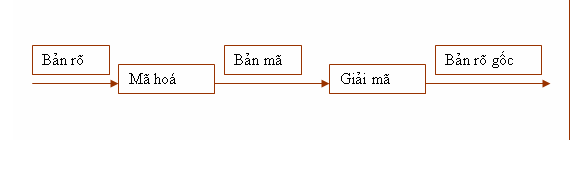
\includegraphics[width=0.5\textwidth]{images/encrypt-decrypt.png}
    \caption{Quy trình mã hóa và giải mã}
    \label{fig:encrypt-decrypt}
\end{figure}

Tính chất cơ bản của mật mã:
\begin{itemize}
    \item[-] Tính bí mật: đảm báo tính bí mật của dữ liệu mà mình gửi đi và
        chỉ những người nắm giữ khóa mới có thể đọc được nội dung.
    \item[-] Tính toàn vẹn: đảm bảo dữ liệu không bị mất mát hoặc chỉnh sửa 
    trong quá trình gửi và nhận mà không bị phát hiện.
    \item[-] Tính xác thực: đảm bảo danh tính của thực thể được xác minh.
    \item[-] Tính không thể chối từ:  đảm bảo người gửi không thể phủ nhận
    thông tin mình gửi đi.
\end{itemize}


\subsubsection{Các loại hệ mật mã}
Các hệ mật mã được chia thành hai loại chính: 
\begin{itemize}
    \item[-] Hệ mật mã đối xứng
    \item[-] Hệ mật mã bất đối xứng
\end{itemize}

a) Hệ mật mã đối xứng

Mật mã đối xứng là một hệ mật mã sử dụng cùng một khóa để mã hóa và giải mã thông tin.
Vì vậy nên khóa bí mật phải giữ an toàn và không được chia sẻ với bất kỳ ai.

Một số hệ mật mã khóa đối xứng hiện đại hay được sử dụng là DES, AES, RC4, RC5,...

Hệ mật sẽ bao gồm:
\begin{itemize}
    \item[-] Bản rõ (M)
    \item[-] Bản mã (C)
    \item[-] khóa (K)
    \item[-] Mã hóa (E): $C = E(K,M)$
    \item[-] Giải mã (D): $M = D(K,C) = D(K,E(K,M))$
\end{itemize}

Vì dùng trung một khóa nên mật mã đối xứng có một số mặt hạn chế như:
\begin{itemize}
    \item[-] Nếu bị đánh cắp hoặc mất khóa thì thông tin cần gửi sẽ bị lộ
    \item[-] Khóa do bên thứ 3 tạo và phải gửi từ bên người gửi đến người nhận, 
    cần phải có một kênh truyền thông an toàn để truyền khóa. Việc đảm bảo khóa 
    không bị lộ khi truyền đi cũng là vấn đề lớn.
    \item[-] Truyền tin giữa các nhóm nhiều người cần 1 lượng lớn khóa, vì 3 người 
    thì không thể dùng chung khóa, giữa 2 người phải có khóa riêng để đảm bảo rằng
    thông tin truyền đi giữa 2 người không bị lộ cho người thứ 3.
    \item[-] Thông tin truyền đi có thể bị sửa đổi vì không có cơ chế xác thực.    
\end{itemize}

Chính vì những nhược điểm như trên nên hệ mật mã bất đối xứng ra đời.

b) Hệ mật mã bất đối xứng

Hệ mã bất đối xứng (hệ mã khóa công khai) là hệ mật mã sử dụng hai khóa khác nhau để mã hóa và giải mã thông tin.
Khóa công khai dùng để mã hóa thông tin và khóa bí mật dùng để giải mã thông tin. Khóa công khai được công khai 
cho tất cả mọi người, còn khóa bí mật thì người nhận nắm giữ.


Hệ mật sẽ bao gồm:
\begin{itemize}
    \item[-] Bản rõ (M)
    \item[-] Bản mã (C)
    \item[-] Khóa (K): 
        \\+ Khóa công khai ($K_{pub}$)
        \\+ Khóa bí mật ($K_{pri}$) 
    \item[-] Mã hóa (E): $C = E(K_{pub},M)$
    \item[-] Giải mã (D): $M = D(K_{pri},C) = D(K_{pri},E(K_{pub},M))$
\end{itemize}

Một số phương pháp sử dụng để trao đổi khóa trong có hệ mật là:
\begin{itemize}
    \item[-] Trao đổi khóa Diffie-Hellman
    \item[-] Trao đổi khóa RSA
    \item[-] Trao đổi khóa ElGamal
\end{itemize}

Trong khóa luận này, em sẽ tập trung vào trao đổi khóa Diffie-Hellman.
\subsection{Trao đổi khóa Diffie-Hellman}

Thuật toán trao đổi khóa Diffie-Hellman giải quyết tình huống sau. Alice và
Bob muốn chia sẻ một khóa bí mật để sử dụng trong mật mã đối xứng, nhưng
phương thức liên lạc của họ không an toàn. Mọi thông tin mà họ trao
đổi đều được quan sát bởi Eve - kẻ tấn công. Làm sao để Alice và Bob có
thể chia sẻ khóa mà Eve không biết? Độ khó của bài toán logarit rời
rạc trong $\mathbb{F}^*_p$ đã đưa ra một giải pháp.

% Thuật toán Trao đổi khóa Diffie - Hellman được tóm tắt ở bảng sau

% \begin{tabular}{|c|c|}
% 	\hline
% 	\multicolumn{2}{Tạo tham số công khai}                                                                                                     \\
% 	\hline
% 	\multicolumn{2}{c}{Một bên chọn và công khai một số nguyên tố $p$ (lớn) và một số nguyên $g$ có bậc nguyên tố lớn trong $\mathbb{F}^*_p$}. \\
% 	\hline
% 	\hline
% 	\multicolumn{2}{c}{Thực hiện tính toán bí mật}                                                                                             \\
% 	Alice                         & Bob                                                                                                        \\
% 	\hline
% 	Chọn bí mật một số nguyên $a$ & Chọn bí mật một số nguyên $b$                                                                              \\
% 	Tính $A \equiv g^a \pmod{p}$  & Tính $B \equiv g^b \pmod{p}$                                                                               \\
% 	\hline
% 	\hline
% 	\multicolumn{2}{c}{Trao đổi giá trị công khai}                                                                                             \\
% 	Alice gửi $A$ cho Bob         & $\longrightarrow A$                                                                                        \\
% 	$B \longleftarrow$            & Bob gửi $B$ cho Alice                                                                                      \\
% 	\hline
% 	\hline
% 	\multicolumn{2}{c}{Tiếp tục thực hiện tính toán bí mật}                                                                                    \\
% 	Alice                         & Bob                                                                                                        \\
% 	\hline
% 	Tính $B^a \pmod{p}$           & Tính $A^b \pmod{p}$                                                                                        \\
% 	Khóa bí mật của cả hai là giá trị $B^a \equiv (g^b)^a \equiv g^{ab} \equiv (g^a)^b \equiv A^b \pmod{p}$
% \end{tabular}

Đầu tiên, Alice và Bob thống nhất sử dụng một số nguyên tố $p$ và một số nguyên khác không $g$  theo modulo $p$. 
Tiếp theo, Alice bí mật chọn một số nguyên $a$ và không cho ai biết. Cùng lúc đó, Bob cũng bí mật chọn một số nguyên $b$.
Alice và Bob sử dụng những số bí mật của họ và tính
$$\underbrace{A \equiv g^a \pmod{p}}_{\text{Alice tính}} \text{ và } \underbrace{B \equiv g^b \pmod{p}}_{\text{Bob tính}}$$

Sau đó, họ trao đổi với nhau giá trị vừa tính được, Alice gửi $A$ cho Bob và Bob gửi $B$ cho Alice. 
Cuối cùng, Bob và Alice tiếp tục sử dụng những số bí mật mà họ đã chọn ở bước trước đó, và tính
$$\underbrace{A' \equiv B^a \pmod{p}}_{\text{Alice tính}} \text{ và } \underbrace{B' \equiv A^b \pmod{p}}_{\text{Bob tính}}$$

$A'$ và $B'$, là bằng nhau, vì:
$$A' \equiv B^a \equiv (g^a)^b \equiv g^{ab} \equiv (g^b)^a \equiv A^b \equiv B' \pmod{p}$$

Giá trị này là khóa mà cả hai cùng chấp nhận sử dụng.

Kẻ tấn công biết được giá trị $p,g,g^a \mod p, g^b \mod p $ nhưng không 
tính toán được khóa $k = g^{ab} \mod p$. Đây là một bài toán khó giải 
trong thời gian đa thức. \cite{elliptic}

\subsection{Mật mã đường cong elliptic}
\subsubsection{Khái niệm đường cong elliptic}

Một \textit{đường cong Elliptic} là tập nghiệm của một phương trình có dạng
$$Y^2 = X^3 + AX + B$$ cùng với một điểm $\mathcal{O}$ ở vô cùng, trong đó hằng số $A$ và $B$ thỏa mãn
$$ 4A^3 + 27B^2 \neq 0$$
Các phương trình thuộc loại này được gọi là \textit{phương trình Weierstrass}. 
Đồ thị của đường cong elliptic có dạng đối xứng qua trục hoành. \cite{elliptic}

Điểm $\mathcal{O}$ là điểm đặc biệt của đường cong elliptic, nó không thuộc đường cong.
Khi ta cộng điểm $P$ với một điểm $P'$ đối xứng với $P$ qua đường cong thì ta có:

$$ P \oplus P' = \mathcal{O}$$

Hai ví dụ cho đường cong elliptic:
$$ E_1: Y^2=X^3-3X+3 $$ và $$ E_2: Y^2=X^3-5X+5 $$ được minh họa ở \hyperref[fg:fg1]{Hình I.2}

\begin{figure}[H]

	\label{fg:fg1}
	\begin{minipage}{0.4\textwidth}
		\centering
		\begin{tikzpicture}[scale = 0.5, line cap=round,line join=round,>=triangle 45,x=1cm,y=1cm]
			\begin{axis}[
					x=1cm,y=1cm,
					axis lines=middle,
					xmin=-5.912600967627929,
					xmax=5.112504977805202,
					ymin=-5.000000419005899,
					ymax=5.000000419005899,
					xtick={-5,-4,...,5},
					ytick={-5,-4,...,5},]
				\clip(-5.912600967627929,-5.000000419005899) rectangle (10.112504977805202,5.000000419005899);
				\draw[line width=2pt,color=blue,smooth,samples=100,domain=-2.1038033040947663:10.112504977805202] plot(\x,{sqrt((\x)^(3)-3*(\x)+3)});
				\draw[line width=2pt,color=blue,smooth,samples=100,domain=-2.1038033040947663:10.112504977805202] plot(\x,{0-sqrt((\x)^(3)-3*(\x)+3)});
			\end{axis}
		\end{tikzpicture}
	\end{minipage}
	\hfill
	\begin{minipage}{0.4\textwidth}
		\centering
		\begin{tikzpicture}[scale = 0.5, line cap=round,line join=round,>=triangle 45,x=1cm,y=1cm]
			\begin{axis}[
					x=1cm,y=1cm,
					axis lines=middle,
					xmin=-5.912600967627929,
					xmax=5.112504977805202,
					ymin=-5.000000419005899,
					ymax=5.000000419005899,
					xtick={-5,-4,...,5},
					ytick={-5,-4,...,5},]
				\clip(-5.912600967627929,-5.000000419005899) rectangle (10.112504977805202,5.000000419005899);
				\draw[line width=2pt,color=blue,smooth,samples=100,domain=-2.791287717641796:0.9999998864501113] plot(\x,{sqrt(abs((\x)^(3)-6*(\x)+5))});
				\draw[line width=2pt,color=blue,smooth,samples=100,domain=1.791293439719924:10.112505461619168] plot(\x,{sqrt(abs((\x)^(3)-6*(\x)+5))});
				\draw[line width=2pt,color=blue,smooth,samples=100,domain=-2.791287717641796:0.9999998864501113] plot(\x,{0-sqrt(abs((\x)^(3)-6*(\x)+5))});
				\draw[line width=2pt,color=blue,smooth,samples=100,domain=1.791293439719924:10.112505461619168] plot(\x,{0-sqrt(abs((\x)^(3)-6*(\x)+5))});
			\end{axis}
		\end{tikzpicture}
	\end{minipage}
	\caption{Đường cong elliptic $E_1$ và $E_2$}
\end{figure}



\subsubsection{Các phép toán trên đường cong elliptic}
a) Phép cộng 

Luật cộng trên $E$ được định nghĩa như sau:

Cho 2 điểm $P$ và $Q$ là 2 điểm thuộc $E$.
$L$ là đường thẳng nối $P$ và $Q$, hoặc là đường tiếp tuyến của $E$ tại $P$ nếu $P=Q$.
Khi đó, giao điểm của $E$ và $L$ là ba điểm $P$, $Q$ và $R$, với $\mathcal{O}$
được hiểu là điểm nằm trên mọi đường thẳng đứng. $R=(a,b)$, tổng của $P$ và $Q$
là điểm $R'=(a,-b)$. Tổng này được ký hiệu là $P \oplus Q$, có thể viết đơn giản $P+Q$.

Luật cộng có thể được minh họa qua hình vẽ sau:

\begin{figure}[H]
	\label{fg:fg2}
	\centering
	\resizebox{0.5\textwidth}{!}{%
	\begin{tikzpicture}[line cap=round,line join=round,>=triangle 45,x=1cm,y=1cm]
		\clip(-5.736430725533388,-5.733053262983473) rectangle (5.923722428745249,5.872549467181578);
		\draw[line width=0.8pt,color=blue,smooth,samples=100,domain=-2.103803291543122:5.923722428745249] plot(\x,{sqrt(abs((\x)^(3)-3*(\x)+3))});
		\draw[line width=0.8pt,color=blue,smooth,samples=100,domain=-2.103803291543122:5.923722428745249] plot(\x,{0-sqrt(abs((\x)^(3)-3*(\x)+3))});
		\draw [line width=0.8pt,domain=-5.736430725533388:5.923722428745249] plot(\x,{(--2.3486301286669415-0.40680839258599555*\x)/1.3559822370127241});
		\draw [line width=0.8pt,dotted] (1.4459883083356893,-1.9982396827947813)-- (1.4459883083356893,1.9982396827947813);
		\begin{scriptsize}
			\draw[color=black] (-1.9451762496392822,0.28794979855338965) node {$E$};
			\draw [fill=black] (0,1.7320508075688772) circle (2pt);
			\draw[color=black] (0.2232031088756924,1.9926505521028977) node {$Q$};
			\draw [fill=black] (-1.3559822370127241,2.1388592001548727) circle (2pt);
			\draw[color=black] (-1.1405574939639143,2.4017787329547793) node {$P$};
			\draw[color=black] (-5.463678604965468,2.8700487609709) node {$L$};
			\draw [fill=black] (1.4459883083356893,1.2982396827947813) circle (2pt);
			\draw[color=black] (1.777890196112844,1.5698847652226198) node {$\ R$};
			\draw [fill=black] (1.4459883083356893,-1.2982396827947813) circle (2pt);
			\draw[color=black] (2.4324952854758553,-1.0348979862010284) node {$R' = P \oplus Q$};
		\end{scriptsize}
	\end{tikzpicture}
	}%
	\caption{Phép cộng trên đường cong elliptic}
\end{figure}

Nếu ta muốn cộng điểm $P$ với chính nó, thì ta lấy đường thẳng L là tiếp tuyến của đồ thị
qua điểm $P$.

Kết quả được minh họa trong hình vẽ sau:

\begin{figure}[H]
	\label{fg:fg3}
	\centering
	\resizebox{0.5\textwidth}{!}{%
	\begin{tikzpicture}[line cap=round,line join=round,>=triangle 45,x=1cm,y=1cm]
		\clip(-5.736430725533388,-5.733053262983473) rectangle (5.923722428745249,5.872549467181578);
		\draw[line width=0.8pt,color=blue,smooth,samples=100,domain=-2.103803291543122:5.923722428745249] plot(\x,{sqrt(abs((\x)^(3)-3*(\x)+3))});
		\draw[line width=0.8pt,color=blue,smooth,samples=100,domain=-2.103803291543122:5.923722428745249] plot(\x,{0-sqrt(abs((\x)^(3)-3*(\x)+3))});
		\draw [line width=0.8pt,domain=-5.736430725533388:5.923722428745249] plot(\x,{(-0.011820467984078764-0.0023798531917433863*\x)/-0.0040177629872759635});
		\draw [line width=0.8pt,dotted] (3.06684049847989,-5.458642606222206)-- (3.06684049847989,5.458642606222206);
		\begin{scriptsize}
			\draw[color=black] (-1.9451762496392822,0.28794979855338965) node {$E$};
			\draw [fill=black] (-1.36,2.1364793469631294) circle (2pt);
			\draw [fill=black] (-1.3559822370127241,2.1388592001548727) circle (2pt);
			\draw[color=black] (-1.1405574939639143,2.4017787329547793) node {$P$};
			\draw[color=black] (-5.463678604965468,-0.10754077627009614) node {$L$};
			\draw [fill=black] (3.06684049847989,4.758642606222206) circle (2pt);
			\draw[color=black] (3.400765313491976,5.020199090406824) node {$\ R$};
			\draw [fill=black] (3.06684049847989,-4.758642606222206) circle (2pt);
			\draw[color=black] (4.0553704028549875,-4.4988499174136285) node {$R' = P \oplus P = 2P$};
		\end{scriptsize}
	\end{tikzpicture}
	}%
	\caption{Phép cộng điểm P với chính nó}
\end{figure}


\begin{theorem}[Thuật toán cộng đường cong Elliptic]
	\label{th:th2}
	Cho
	$$E:Y^2 = X^3 + AX + B$$
	là một đường cong elliptic và $P_1$  và $P_2$ là hai điểm trên $E$.
	\begin{enumerate}
		\item Nếu $P_1 = \mathcal{O}$ thì $P_1 + P_2 = P_2$.
		\item Ngược lại, nếu $P_2 = \mathcal{O}$ thì $P_1 + P_2 = P_1$.
		\item Ngược lại, viết $P_1 = (x_1, y_2)$ và $P_2 = (x_2, y_2)$.
		\item Nếu $x_1 = x_2$ và $y_1 = -y_2$ thì $P_1 + P_2 = \mathcal{O}$.
		\item Nếu không, định nghĩa $\lambda$ bởi
		      $$ \lambda = \begin{cases}
				      \frac{y_2-y_1}{x_2 - x_1} & \text{nếu } P_1 \neq P_2 \\
				      \frac{3x_1^2 + A}{2y_1}   & \text{nếu } P_1 = P_2.
			      \end{cases} $$
		      Và ta có $P_1 + P_2 = (x_3, y_3)$, trong đó:
		      $$x_3 = \lambda^2 - x_1 - x_2 \ \ \  \text{ và } \ \ \  y_3 = \lambda(x_1 - x_3) - y_1.$$
	\end{enumerate}
\end{theorem}


b) Phép nhân

Phép nhân $P$ với một số nguyên $n$ được định nghĩa bởi 
$$nP = P + P + \cdots + P$$
với $n$ lần phép cộng.

\subsubsection{Đường cong elliptic trên trường hữu hạn}
Các ứng dụng về mật mã của đường cong Elliptic đa số chỉ sử dụng các đường cong trên
trường hữu hạn.

\begin{definition}
    	Trường là một tập hợp K có nhiều hơn một phần tử, được định nghĩa hai phép toán cộng và nhân,
    	ký hiệu bởi dấu $(+)$ và dấu $(.)$. Trường thỏa mãn các tính chất của số học.
\end{definition}

\begin{definition}
	Trường hữu hạn (còn gọi là trường Galois) là những trường có hữu hạn số phần tử.
	Bậc của một trường hữu hạn là số phần tử của nó, là số nguyên tố hoặc lũy thừa nguyên tố.
\end{definition}
Trường hữu hạn là cơ bản trong một số lĩnh vực toán học và khoa học máy tính,
bao gồm lý thuyết số, hình học đại số, lý thuyết Galois, hình học hữu hạn, mật mã và lý thuyết mã hóa.

Đường cong elliptic $E$ trên trường hữu hạn $\mathbb{F}_q$ là một phương trình có dạng:
$$E: Y^2 = X^3 + AX + B\ \text{với các hằng số}\ A, B \in F_p\ \text{thỏa mãn}\ 4A^3 + 27B^2 \neq 0$$

Tập hợp các điểm trên $E$ có tọa độ thuộc $\mathbb{F} _p$ được kí hiệu bởi
$$E(F_p) = \{(x, y) : x, y \in \mathbb{F}_p\ \text{thỏa mãn}\ y^2 = x^3 + A x + B\} \cup \mathcal{O}$$

\subsubsection{Khái niệm mật mã đường cong elliptic}
Mật mã đường cong elliptic (ECC) 
là một phương pháp mã hóa và giải mã thông tin bằng cách sử dụng các 
điểm trên đường cong elliptic. ECC được sử dụng để đảm bảo tính bảo 
mật và an toàn trong các ứng dụng mật mã, như mã hóa thông tin, xác thực người dùng, và tạo chữ ký số.

Trao đổi khóa Diffie - Hellman trên elliptic, thay thế bài toán logarit rời
rạc cho trường hữu hạn $F_p$ bằng bài toán logarit rời rạc cho đường cong elliptic $E(F_p)$.
Đây là các bài toán khó có thể giải quyết trong thời gian đa thức. Phù 
hợp để sử dụng trong các ứng dụng mật mã.

a) Trao đổi khóa Diffie - Hellman trên đường cong elliptic

	Alice và Bob cùng đồng ý sử dụng một đường cong elliptic $E (\mathbb{F}_p)$ và một điểm $P \in E (\mathbb{F}_p)$.
	Alice bí mật chọn một giá trị $n_A$, Bob chọn một giá trị $n_B$. Cả hai sử dụng số bí mật của họ và tính
$$\underbrace{Q_A = (n_AP)}_{\text{Alice tính}} \text{ và } \underbrace{Q_B = (n_BP)}_{\text{Bob tính}}$$

Sau đó, họ trao đổi với nhau giá trị vừa tính được, Alice gửi $Q_A$ cho Bob và Bob gửi
$Q_B$ cho Alice. Sau đó tính $n_A Q_B$ và $ n_BQ_A $.
Và họ có khóa bí mật chung
$$ n_AQ_B = (n_An_B)P = n_BQ_A,$$

Giống như bài toán logarit rời rạc trên trường hữu hạn, bài toán logarit rời rạc trên đường cong elliptic 
cũng là một bài toán khó. 

Hiện nay, thuật toán phổ biến để giải quyết bài toán logarit rời rạc 
trên đường cong elliptic là thuật toán Pollard's rho và thuật toán 
đặc biệt hơn là thuật toán số học đại số đường cong elliptic (ECDLP).

Thuật toán Pollard's rho được sử dụng để tìm giá trị bí mật của 
logarit rời rạc trên đường cong elliptic bằng cách sử dụng phép 
nhân trên đường cong để tìm kiếm các chu kỳ lặp lại. Thuật toán này 
có độ phức tạp tính toán khoảng $O(\sqrt n)$, trong đó $n$ là số lượng 
phần tử trong đường cong.

Vậy nên để đảm bảo độ bảo mật và tính khó tính toán cho bài toán trên,
ta sử dụng đường cong elliptic có số phần tử lớn, hay chọn $p$ là một
số nguyên tố lớn, và chọn 1 đường cong elliptic trên trường hữu hạn $F_p$. \cite{elliptic}

\subsection{Mật mã đường cong elliptic trong chữ ký số}
\subsubsection{Chữ ký số} 

Chữ ký số là một phương pháp xác thực nguồn gốc và tính toàn vẹn của tài liệu điện tử hoặc thông tin truyền qua mạng. 

Theo quy định của pháp luật và căn cứ vào Khoản 6 Điều 3 Nghị định 130/2018 NĐ-CP nêu rõ: 

`` “Chữ ký số” là một dạng chữ ký điện tử được tạo ra bằng sự biến đổi một thông điệp dữ liệu sử dụng hệ thống mật mã không đối xứng, theo đó, người có được thông điệp dữ liệu ban đầu và khóa công khai của người ký có thể xác định được chính xác:

a) Việc biến đổi nêu trên được tạo ra bằng đúng khóa bí mật tương ứng với khóa công khai trong cùng một cặp khóa;

b) Sự toàn vẹn nội dung của thông điệp dữ liệu kể từ khi thực hiện việc biến đổi nêu trên.”

Khi người tạo chữ ký số ký một tài liệu điện tử, phần mềm tạo chữ ký số sẽ sử dụng khóa bí mật để tạo ra một \textbf{mã hóa dữ liệu} đính kèm vào tài liệu đó. \textbf{mã hóa dữ liệu}  này bao gồm các thông tin về chữ ký số, bao gồm cả khóa công khai của người tạo chữ ký. Khi người nhận tài liệu muốn xác thực chữ ký số, phần mềm xác thực chữ ký số sẽ sử dụng khóa công khai để giải mã mã hóa dữ liệu và kiểm tra tính toàn vẹn của tài liệu đó.

Chữ ký số được sử dụng rộng rãi trong các ứng dụng như giao dịch thương mại điện tử, xác thực người dùng và chữ ký điện tử. Nó giúp đảm bảo tính toàn vẹn và xác thực của thông tin truyền qua mạng và giảm thiểu rủi ro về gian lận và giả mạo.

\subsubsection{Chữ ký số trên đường cong elliptic}
\label{sec:ecdsa}

Chữ ký số trên đường cong elliptic (ECDSA) là một phương pháp mã hóa và giải mã thông tin bằng cách sử dụng các điểm trên đường cong elliptic. ECDSA được sử dụng để đảm bảo tính bảo mật và an toàn trong các ứng dụng mật mã, như mã hóa thông tin, xác thực người dùng, và tạo chữ ký số.

Chữ ký số trên đường cong elliptic được sử dụng nhiều bởi bài toán logarit rời
rạc cho đường cong elliptic khó hơn rất nhiều so với bài toán logarit rời rạc cho $F^*_p$.

Giả sử rằng Alice muốn gửi một tin nhắn $m$ để Bob. Bob cần xác minh biết chắc chắn tin nhắn đó đến từ Alice. 

Giao thức ECDSA hoạt động như sau:

Alice và Bob cùng đồng ý sử dụng một đường cong elliptic $E (\mathbb{F}_p)$ và một điểm $G \in E (\mathbb{F}_p)$.
Hai người cũng cùng sử dụng 1 hàm băm H.

Các giá trị công khai là a,b,G,p.

\textbf{Bước 1: Thuật toán sinh khóa} 
Alice bí mật chọn một giá trị $n_A$.

Alice tạo private key: $n_A$.

Alice tạo public key: $P = n_AG$.

\textbf{Bước 2: Thuật toán tạo chữ ký} 
\begin{enumerate}

	\item Alice chọn một số $k$ sao cho $1 \le k \le p-1$.
	\item Alice tính $K = (x_p, y_p) =  kG$.
	\item Alice tính $r =  x_P \mod p$ , nếu $r = 0$ thì quay lại\textbf{ 2.1}.
	\item Alice tính $e = H(m)$
	\item Alice tính $s = k^{-1}(e+ n_A r)\mod p$, $n_A$ là khóa bí mật của Alice và $k^{-1}$ là nghịch đảo modulo $p$ của $k$.\\
	      Nếu $s = 0$ thì trở lại \textbf{2.1}.                          
	\item  Cặp  chữ ký ($r, s$) được tạo thành.
\end{enumerate}
Alice gửi đi bộ chữ ký $(r,s)$ cùng thông điệp $m$ cho Bob.

\textbf{Bước 2: Thuật toán xác minh chữ ký} 
\begin{enumerate}

	\item Bob tính $e = H(m)$
	\item Bob tính $ w = s^{-1} \mod p$.
	\item Bob tính $u_1 =  e \times w \mod p$ và $u_2 =  r \times w \mod p$.
	\item Bob tính $X =(x_1,y_1)= u_1G + u_2P$.
	\item Nếu $X = 0$, thì từ chối chữ ký, nếu không thì $v = x_1 \mod p$.
	\item Nếu $v=r$ thì chấp nhận chữ ký, nếu không thì từ chối chữ ký.
\end{enumerate}

\textbf{Tính đúng đắn của thuật toán}

Ta có:

$s = k^{-1}(e+ n_A r)\mod p$

$\to k = s^{-1}(e+ n_A r)\mod p$

$= w \times e + w \times n_A \times r \mod p$

$=u_1 + u_2 \times n_A \mod p$

$\to u_1G + u_2P = u_1G + u_2 \times n_A G = (u_1+u_2 \times n_A)G = kG$

Nếu chữ ký trên đúng thì $X=K$ hay $v=r$. \cite{elliptic}



Chữ ký số có ý nghĩa to lớn và trở thành một phần không thể thiếu đối
với ngành mật mã học. Ứng dụng của chữ ký số đã được triển khai trên 
nhiều quốc gia trên thế giới, trong đó có Việt Nam. So với chữ ký tay, 
chữ ký số giúp các cá nhân, doanh nghiệp thực hiện việc ký các tài 
liệu được nhanh chóng, hiệu quả hơn. 

Hiện nay ECDSA đang được sử dụng rộng rãi, đặc biệt trong công nghệ Blockchain. 

\section{Cây Merkle}
\subsection{Khái niệm cây Merkle}

Merkle Tree là một cấu trúc dữ liệu cây nhị phân được sử dụng trong một số loại hệ thống phân 
tán để đảm bảo tính toàn vẹn dữ liệu. 

Cấu trúc Merkle Tree là một cấu trúc dữ liệu cây nhị phân, trong đó mỗi nút lá của cây biểu diễn
một khối dữ liệu và mỗi nút cha của hai nút lá biểu diễn giá trị băm của hai khối dữ 
liệu liên tiếp. Các giá trị băm này được tính toán bằng cách sử dụng một thuật toán băm như 
SHA-256 hoặc SHA-3.


\begin{figure}[h]
    \centering
    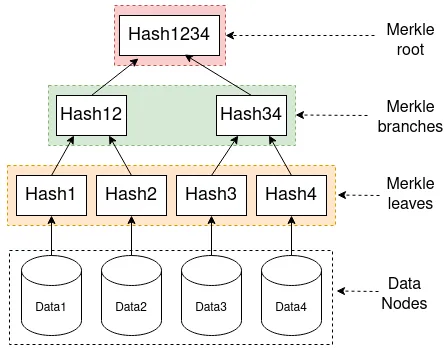
\includegraphics[width=0.6\textwidth]{images/Merkle_Tree.png}
    \caption{Merkle Tree }
    \label{fig:merkle_tree}
\end{figure}

Các giá trị băm của các cặp khối dữ liệu liên tiếp được sử dụng để tính toán giá trị băm của 
các nút cha tiếp theo. Quá trình này được lặp lại cho đến khi chỉ còn lại một giá trị băm duy 
nhất, được gọi là "root hash". Các giá trị băm này được sử dụng để đảm bảo tính toàn vẹn của 
dữ liệu được lưu trữ trong cây.

Số nút lá của cây Merkle là luỹ thừa của 2 (2,4,8,16,32,...). Nếu số nút lá của cây không
đủ, thì sẽ sử dụng dữ liệu cuối cùng để đại diện cho khối dữ liệu còn thiếu.



Một cây Merkle có thể được sử dụng để giảm thiểu khối lượng dữ liệu cần truyền qua mạng khi 
xác minh tính toàn vẹn của một tập hợp lớn các khối dữ liệu. Thay vì truyền toàn bộ dữ liệu qua
mạng, chỉ cần truyền giá trị băm của các khối dữ liệu và giá trị băm của các nút cha để xác minh tính toàn vẹn của dữ liệu.

Một trong những ứng dụng phổ biến nhất của cây Merkle là trong blockchain. Trong blockchain,
các giao dịch được kết hợp với nhau để tạo thành một khối, và các khối này được kết hợp với nhau 
để tạo thành một cây Merkle. Các thợ đào sẽ sử dụng giá trị băm của cây Merkle để xác minh tính 
toàn vẹn của khối, giúp ngăn chặn các giao dịch giả mạo hoặc thay đổi dữ liệu trên blockchain.


\subsection{Merkle Root}

Merkle Root là giá trị băm  của nút gốc trong cây Merkle. Nó được tính toán 
bằng cách kết hợp giá trị băm của các nút cha trong cây Merkle.

Trong blockchain, Merkle Root được sử dụng để đại diện cho tất cả các giao dịch trong một khối. 
Các giao dịch được kết hợp với nhau để tạo thành một cây Merkle, và Merkle Root của cây này 
được sử dụng để đại diện cho toàn bộ khối trong blockchain.

Việc sử dụng Merkle Root giúp tăng tính toàn vẹn và bảo mật của blockchain. Nếu một giao dịch trong khối bị thay đổi, thì giá trị băm của Merkle Root sẽ thay đổi và blockchain sẽ không chấp nhận khối này. Do đó, Merkle Root giúp ngăn chặn các cuộc tấn công như giao dịch giả mạo hoặc thay đổi dữ liệu trên blockchain.

\subsection{Xác minh trong cây Merkle }

Chúng ta xác minh các giao dịch trên cây Merkle như thế nào?

Giả sử chúng ta có một cây Merkle với 8 nút lá thể hiện các giao dịch từ A đến H. Chúng ta sẽ sử dụng giá trị băm 
của các nút lá để xác minh tính toàn vẹn của dữ liệu. Giá trị băm của các nút lá 
được sử dụng để tính toán giá trị băm của các nút cha, và quá trình này được lặp 
lại cho đến khi chỉ còn lại một giá trị băm duy nhất, được gọi là ``root hash". 

\begin{figure}[h]
    \centering
    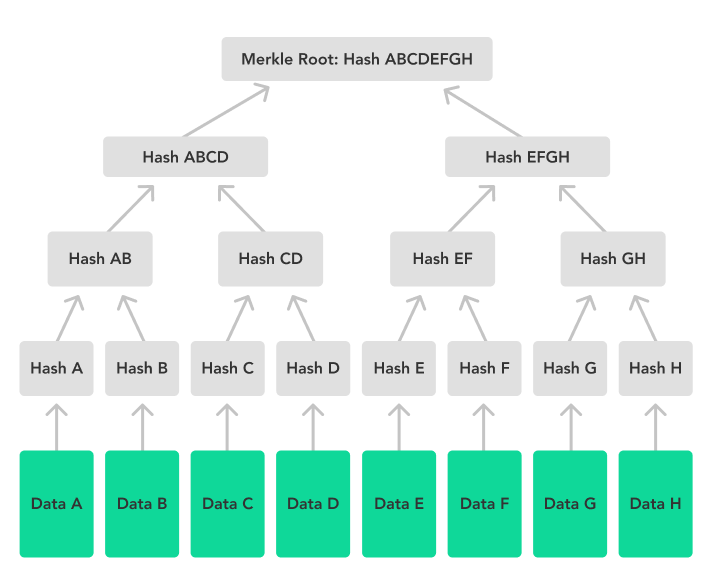
\includegraphics[width=0.6\textwidth]{images/merkle-tree-8levels.png}
    \caption{Cây Merkle 8 lá}
    \label{fig:merkle_tree_8levels}
\end{figure}


Giả sử ta cần xác minh một giao dịch, đầu tiên ta băm giao dịch và tìm kiếm kết quả
trong cây Merkle, nếu không tìm thấy kết quả thì thông tin giao dịch là giả. Nếu tìm được
một hàm băm lá trùng khớp với hàm băm ta vừa tính toán, thì thực hiện tính toán Merkle Root. 

Giả sử hàm băm thông tin giao dịch cần xác minh trùng khớp với Hash D.
Ta lấy thông tin Hash C để tính được Hash CD, sau đó lấy thông tin Hash AB để tính được Hash ABCD.
Cuối cùng sử dụng thông tin Hash EFGH kết hợp với Hash ABCD để tính được Merkle Root.

Cuối cùng so sánh Merkle Root vừa tính với giá trị Merkle Root được lưu trữ trong 
cây Merkle. Nếu hai giá trị này giống nhau, thì giao dịch là đúng, nếu không thì thông tin
giao dịch là giả.


\section{Blockchain}
\subsection{Khái niệm Blockchain}
\label{subsec:khainiemblockchain}
Blockchain là một công nghệ mới và đầy tiềm năng, được sử dụng để lưu 
trữ và quản lý thông tin một cách an toàn và minh bạch. Nó là một cơ 
sở dữ liệu phân tán, trong đó dữ liệu được lưu trữ trên nhiều nút 
mạng và được bảo vệ bởi mã hóa mạnh. Cơ sở dữ liệu này sẽ lưu thông tin trong các khối , các khối 
này sẽ được liên kết với nhau bằng mã hóa và có thể mở rộng theo 
thời gian để tạo thành chuỗi .Vì vậy, 
nếu một khối bị thay đổi hoặc xóa, toàn bộ chuỗi sẽ bị ảnh 
hưởng và trở nên không hợp lệ.

Ta có thể hiểu đơn giản Blockchain chính là một cuốn sổ cái kỹ thuật 
số phân tán. Cuốn sổ cái này sẽ lưu trữ tất cả các loại thông tin 
giao dịch và được sao chép thành nhiều bản đặt tại nhiều máy tính khác nhau. 

Không giống như các cơ sở dữ liệu thông thường, blockchain là cơ sở dữ liệu phi tập trung. 
Tức là blockchain không đặt tại một vị trí nhất định và chịu sự quản lý của một quản trị viên mà nó được sao chép thành nhiều bản và được lưu trên các máy tính riêng lẻ gọi là nút. 


Một trong những ưu điểm của blockchain là tính minh bạch và an toàn. 
Do dữ liệu được lưu trữ phân tán, không ai có thể can thiệp vào và 
thay đổi dữ liệu một cách dễ dàng.

Tuy nhiên, cũng có những hạn chế của blockchain, bao gồm tốc độ xử 
lý chậm và khó khăn trong việc thay đổi các thông tin đã được lưu 
trữ trên blockchain. Tuy nhiên, với sự phát triển và ứng dụng đa 
dạng, blockchain đang trở thành một công nghệ quan trọng và tiềm 
năng cho tương lai.
\subsection{Hệ thống phi tập chung}

Ở phần \ref{subsec:khainiemblockchain} chúng ta nói rằng Blockchain là một hệ thống 
phi tập trung. Vậy hệ thống phi tập trung khác hệ thống tập trung
như thế nào?

\begin{figure}[h]
    \centering
    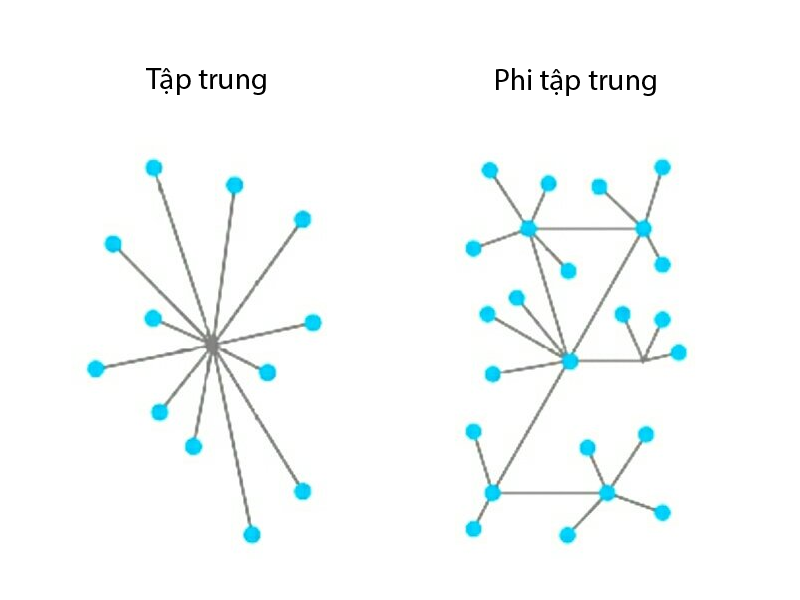
\includegraphics[width=0.7\textwidth]{images/He_thong_tap_chung:phi_tap_chung.png}
    \label{fig:He_thong_tap_chung/phi_tap_chung}
    \caption{Hệ thống tập trung và phi tập trung}
\end{figure}

Hệ thống tập trung là một hệ thống mà tất cả các thành phần của nó
được đặt tại một vị trí và chịu sự quản lý của một quản trị viên.
Ví dụ như hệ thống quản lý thông tin của một công ty, hệ thống
quản lý thông tin của một trường học, hệ thống quản lý thông tin
của một bệnh viện, hệ thống quản lý thông tin của một ngân hàng
v.v...

Hệ thống phi tập trung là một hệ thống mà không có bên nào kiểm soát 
toàn bộ. Trong hệ thống này, tất cả các thực thể trong hệ thống là 
ngang hàng. Các quyết định và hoạt động được phân phối trên nhiều 
thực thể độc lập và được quyết định bởi một cộng đồng người dùng.

Ưu điểm của hệ thống phi tập chung là dữ liệu sẽ được đảm bảo, 
không bị thay đổi, không bị xóa bỏ. Hệ thống phi tập chung đảm bảo
tính minh bạch, an toàn, độ tin cậy và khả năng phát triển dễ dàng.
Tuy nhiên, tốc độ xử lý chậm và khó khăn trong việc đạt được sự đồng
thuận giữa các thực thể phân tán là những vấn đề cần giải quyết để 
hế thống phát triển mạnh mẽ hơn.

\subsection{Cấu tạo của Blockchain}

Một blockchain cơ bản bao gồm các thành phần sau:
\begin{itemize}
    \item[-] Khối: là một đơn vị cơ bản của blockchain, chứa thông tin về các giao dịch và các liên kết đến các block khác trong chuỗi.
    \item[-] Giá trị băm: là một mã hóa duy nhất đại diện cho một khối hoặc một tập hợp các thông tin trên blockchain. Giá trị băm được tạo ra bằng cách sử dụng một thuật toán mã hóa, chẳng hạn như SHA-256.
    \item[-] Chuỗi khối: là một loạt các khối được kết nối với nhau theo thứ tự thời gian. Mỗi khối trong chuỗi chứa liên kết đến khối trước đó và khối sau đó, tạo thành một chuỗi liên kết.
    \item[-] Giao thức đồng thuận: là một phương thức để xác minh và chứng thực các giao dịch trên blockchain. 
    \item[-] Nút: là một thiết bị hoặc một phần mềm chạy trên thiết bị, được sử dụng để tham gia vào mạng blockchain, giúp xác minh và chứng thực các giao dịch.
    \item[-] Ví: là một phần mềm hoặc thiết bị lưu trữ khóa cá nhân và khóa công khai, cho phép người dùng thực hiện các giao dịch trên mạng blockchain.

\end{itemize}

Các thành phần này cùng hoạt động để tạo ra một hệ thống blockchain an toàn, minh bạch và phân tán, giúp các giao dịch trên mạng blockchain được xác minh và chứng thực một cách chính xác.

\subsubsection{Cấu trúc của một khối}


Cấu trúc của 1 khối được minh hoạ qua sơ đồ sau:
\begin{figure}[h]
    \centering
    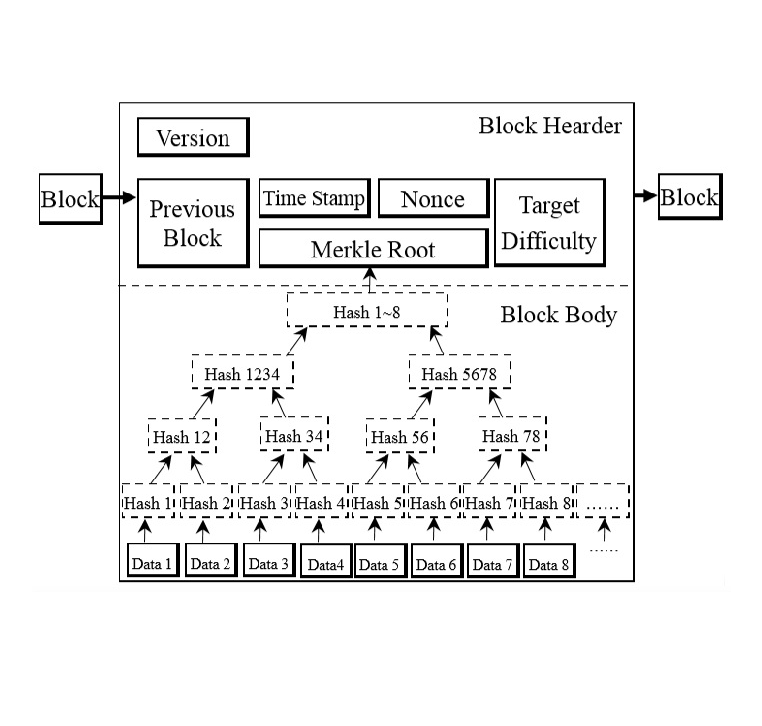
\includegraphics[width=0.8\textwidth]{images/Cau_truc_khoi.png}
    \label{fig:cau_truc_khoi}
    \caption{Cấu trúc của 1 khối}
\end{figure}

\begin{itemize}
    \item[-] Block header: chứa các thông tin về block, bao gồm: thời gian tạo block, hash của block trước đó, hash của block hiện tại, nonce, và các thông tin khác.
    \begin{itemize}
        \item[+] Version: phiên bản của blockchain.
        \item[+] Previous Block: Giá trị băm của block trước.
        \item[+] Time Stamp: Thời gian block này được tạo.
        \item[+] Merkle Root: Mã hash của tất cả các giao dịch trong khối hiện tại, 
        được tính toán bằng cách sử dụng cây Merkle.
        \item[+] Nonce: là một số ngẫu nhiên được sử dụng để giải quyết bài toán PoW.
        \item[+] Target Difficulty: là một giá trị được sử dụng để xác định độ khó của bài toán PoW trong block này.
    \end{itemize}
    \item[-] Block Body: chứa các các giao dịch được thực hiện trên blockchain.
\end{itemize}

\subsection{Các kỹ thuật trong Blockchain}
\subsubsection{Cấu trúc phi tập trung}

Cấu trúc phi tập chung trong blockchain được xây dựng 
để đảm bảo tính an toàn và bảo mật của hệ thống. Cấu trúc này cho phép thông tin được phân tán trên nhiều nút mạng khác nhau, giúp giảm thiểu rủi ro bị tấn công và tăng tính đáng tin cậy.

Cấu trúc phi tập chung trong blockchain có có thành phần cơ bản như:
\begin{itemize}
    \item[-] Mạng ngang hàng: Các nút trong mạng sẽ kết 
    nối với nhau để chia sẻ thông tin và cập nhật các giao dịch mới nhất.
    \item[-] Giao thức đồng thuận: Để đảm bảo tính nhất 
    quán và đáng tin cậy của dữ liệu, các nút trong mạng sẽ phải đồng thuận về 
    sự thay đổi của blockchain. Các giao thức đồng thuận phổ biến bao gồm Bằng chứng công việc (PoW)
     và Bằng chứng cổ phẩn (PoS).
    \item[-] Nút: đóng vai trò xác nhân để các khối mới và xác nhận các giao dịch.
    \item[-] Blockchain: Dữ liệu được lưu trữ trên blockchain, một chuỗi
    các khối được kết nối với nhau theo thứ tự thời gian.
    \item[-] Ví: là một phần mềm hoặc thiết bị lưu trữ khóa cá nhân và
    khóa công khai, cho phép người dùng thực hiện các giao dịch trên mạng
    blockchain.
\end{itemize}

Các thành phần này cùng hoạt động với nhau để tạo ra một hệ thống phi tập trung, 
nơi mà dữ liệu được phân tán trên nhiều nút khác nhau và không có bất kỳ cơ quan 
trung gian nào kiểm soát hoặc giám sát.

\subsubsection{Tính tin cậy}
Tính tin cậy là một trong những điểm mạnh của blockchain. Điều 
này được đảm bảo bởi cấu trúc phi tập trung của hệ thống, nghĩa là không có 
một tổ chức hay cá nhân nào có quyền kiểm soát toàn bộ blockchain. Thay vào đó, 
blockchain được phân tán trên nhiều nút trong mạng, mỗi nút lưu trữ một bản sao 
của toàn bộ blockchain.

Việc phân tán dữ liệu trên nhiều nút khác nhau giúp tăng tính đáng tin cậy của 
hệ thống, vì không có một nút duy nhất nào có thể gian lận hoặc tấn công hệ 
thống. Nếu một nút bị tấn công hoặc lỗi, các nút khác vẫn có thể tiếp tục 
hoạt động và duy trì tính toàn vẹn của blockchain.

\subsubsection{Giao thức đồng thuận}
\begin{itemize}
    \item[-] \textbf{PoW}: có nhiệm vụ đảm bảo 
    tính nhất quán và đáng tin cậy của blockchain bằng cách yêu cầu các nút 
    trong mạng phải thực hiện một số lượng lớn tính toán để xác nhận giao dịch
    và thêm mới các khối vào blockchain. Cụ thể, các nút trong mạng sẽ cạnh 
    tranh với nhau để giải quyết một bài toán tính toán phức tạp, được gọi là 
    "bài toán đào". Bài toán này yêu cầu các nút phải tìm ra một giá trị băm 
    thoả mãn điều kiện, dựa trên các thông tin trong khối mới nhất và khối trước đó. 
    Việc giải quyết bài toán này đòi hỏi sự tiêu tốn của năng lượng tính toán, 
    thời gian và tài nguyên máy tính. Điều kiện này là giá trị “difficulty” – 
    số lượng số 0 đứng phía trước giá trị băm.
    \item[-] \textbf{PoS}: là một giao thức đồng thuận được sử 
    dụng trong blockchain để đảm bảo tính nhất quán và đáng tin cậy của dữ 
    liệu. PoS hoạt động khác với PoW, bằng cách không yêu cầu các nút trong 
    mạng thực hiện các hoạt động tính toán phức tạp để giải quyết bài toán đào, 
    mà thay vào đó, các nút sẽ được chọn để xác nhận giao dịch và thêm mới các 
    khối vào blockchain dựa trên số lượng tiền điện tử mà họ đã có trong tài 
    khoản của mình. Khi lượng tiền điện tử trong ví càng cao thì khả năng được chọn 
    để xác nhận giao dịch càng lớn. Điều này giúp giảm thiểu việc tiêu tốn năng
    lượng tính toán và tài nguyên máy tính, đồng thời tăng tốc độ xác nhận giao
    dịch và thêm mới các khối vào blockchain.
    
\end{itemize}


Blockchain sử dụng các giao thức đồng thuận để đảm tính tin cậy và bảo mật. Khi không nắm được 51\% 
số nút trong mạng, dữ liệu mạng không thể bị kiểm soát và sửa đổi. Do đó, 
bản thân Blockchain đã trở nên tương đối an toàn và có thể tránh việc sửa đổi 
dữ liệu. Vì thế, nếu một số lượng lớn các nút có khả năng tính toán mạnh được 
tham gia vào hệ thống thì dữ liệu trong hệ thống này sẽ có độ bảo mật cao hơn.  



\subsection{Cách thức hoạt động của Blockchain}
\subsubsection{Thêm giao dịch mới vào Blockchain}
Để thêm một giao dịch trong blockchain, quá trình cần phải đi qua các bước sau:
\begin{itemize}
    \item[-] Người dùng gửi một thông tin của giao dịch mới vào mạng blockchain.
    \item[-] Giao dịch mới sẽ được gửi đến tất cả các nút trong mạng blockchain.
    \item[-] Các nút trong mạng sẽ kiểm tra tính hợp lệ của giao dịch bằng cách kiểm tra tính 
    đúng đắn của chữ ký số.
    \item[-] Các giao dịch hợp lệ sẽ được đóng gói lại thành một khối và bao gồm các thông tin 
    như giá trị băm của khối trước, thông tin của giao dịch, phiên bản, thời gian tạo khối,... 
    \item[-] Tính toán giá trị băm của khối mới, các nút trong mạng sẽ xác nhận tính hợp 
    lệ của khối mới. Để xác nhận, các nút sẽ kiểm tra giá trị băm của khối trước đó có khớp 
    với giá trị \textit{Previous Hash} được lưu trong khối mới hay không. Tiếp theo, sẽ kiểm tra \textit{Merkle Root}
    của khối mới có khớp với giá trị \textit{Merkle Root} được lưu trong khối mới hay không. Cuối cùng sẽ 
    kiểm tra thời gian tạo khối, giá trị nonce có hợp lệ hay không. 
    \item[-] Nếu khối mới được xác nhận là hợp lệ, nó sẽ được thêm vào blockchain. Khối mới này sẽ trở thành khối 
    mới nhất trong chuỗi blockchain và các giao dịch được bao gồm trong khối sẽ được coi là đã được xác nhận và 
    lưu trữ trong blockchain.
\end{itemize}

\subsubsection{Xác thực một giao dịch}
\begin{itemize}
    \item[-] Tính giá trị băm của giao dịch cần xác thực.
    \item[-] Tìm tất cả các khối trong chuỗi khối và kiểm tra xem giá trị băm của giao 
    dịch đó có nằm trong danh sách các giao dịch của mỗi khối hay không.
    Nếu không tồn tại thì thông tin giao dịch là sai.
    \item[-] Nếu có thì kiểm tra tính toàn vẹn của giao dịch bằng cách sử dụng chữ ký số 
    của người gửi giao dịch.
        \item[+] Sử dụng khoá công khai để giải mã chữ ký số.
        \item[+] Tính toán lại giá trị băm của dữ liệu giao dịch bằng cách sử dụng cùng
        thuật toán mã hóa được sử dụng trong blockchain.
        \item[+] So sánh hai giá trị vừa tính được. Nếu trùng khớp thì giao dịch được
        xác nhận là hợp lệ và tính toàn vẹn của giao dịch được xác định.
        Việc xác minh tính toàn vẹn trên dựa vào thuật toán Chữ ký số trên đường cong 
        elliptic (ECDSA) đã được chứng minh ở phần \textbf{2.4.2}
\end{itemize}

\subsection{Các ứng dụng điển hình của Blockchain}
\subsubsection{Tiền số}

Tiền số trong blockchain là một loại tiền tệ số được tạo ra và quản lý bởi các 
mạng blockchain, được mã hóa để đảm bảo tính bảo mật và độ tin cậy của các giao 
dịch trên mạng. Các ví dụ tiêu biểu của tiền số trên thế giới hiện nay bao gồm 
Bitcoin, Ethereum, Litecoin, Ripple và Bitcoin Cash. Mỗi loại tiền số có đặc điểm 
và tính năng riêng, tuy nhiên tất cả đều được tạo ra và quản lý bởi các mạng 
blockchain. Tiền số trong blockchain có tính năng phân quyền, không có bên trung 
gian nào can thiệp hoặc kiểm soát quá trình giao dịch và các giao dịch được xác 
thực bởi các nút trong mạng. Tiền số trong blockchain được sử dụng trong nhiều 
ứng dụng như chuyển tiền, thanh toán trực tuyến, đầu tư và trao đổi trên các sàn 
giao dịch tiền số, tuy nhiên, nó cũng đang gặp phải một số thách thức như tính 
ổn định giá, độ tin cậy và sự phức tạp về quy định pháp lý.

\subsubsection{Hợp đồng thông minh} 

Hợp đồng thông minh là một chương trình tự động được viết bằng ngôn ngữ lập trình và thực thi trên mạng blockchain. Chúng được thiết kế để tự động thực hiện các điều khoản hợp đồng một cách đáng tin cậy, không cần phải dựa vào bên thứ ba.

Hợp đồng thông minh được định nghĩa bởi một tập hợp các quy tắc và điều kiện mà khi được kích hoạt, nó sẽ tự động thực hiện các hành động được yêu cầu. Các hợp đồng thông minh được sử dụng để thực hiện các giao dịch tài chính, quản lý quy trình kinh doanh, bảo vệ sở hữu trí tuệ và quản lý dữ liệu.

Một trong những đặc điểm của hợp đồng thông minh là tính bảo mật cao, vì chúng được mã hóa và lưu trữ trên mạng blockchain, không thể bị can thiệp hay thay đổi bởi bất kỳ ai. Các giao dịch được thực hiện thông qua các hợp đồng thông minh cũng được xác thực và đảm bảo tính đúng đắn bởi các nút trong mạng.

Hợp đồng thông minh đã được triển khai trong nhiều lĩnh vực, bao gồm tài chính, bảo hiểm, bất động sản, quản lý chuỗi cung ứng và nhiều lĩnh vực khác. Tuy nhiên, việc triển khai hợp đồng thông minh vẫn đang đối mặt với một số thách thức, bao gồm khả năng lập trình và kiểm tra hợp đồng, độ tin cậy và quy định pháp lý.
\chapter{Truy xuất nguồn gốc thực phẩm}
\section{Khái niệm truy xuất nguồn gốc thực phẩm}
\subsection{Giới thiệu}

Truy xuất nguồn gốc thực phẩm là quá trình xác định nguồn gốc và lịch sử sản xuất
của một sản phẩm thực phẩm từ giai đoạn sản xuất đến khi đến tay người tiêu dùng. Ý
nghĩa của việc truy xuất nguồn gốc thực phẩm là giúp người tiêu dùng đảm bảo được
an toàn về chất lượng và nguồn gốc của sản phẩm mà mình sử dụng, đồng thời cũng là
một phương tiện quan trọng giúp kiểm soát và ngăn chặn sự xuất hiện của những sản
phẩm thực phẩm giả mạo, không rõ nguồn gốc và an toàn.

Việc truy xuất nguồn gốc thực phẩm đang được xem là một xu hướng quan trọng
trong ngành thực phẩm, đặc biệt là trong bối cảnh ngày nay, khi mối đe dọa về an toàn
thực phẩm và việc giả mạo sản phẩm thực phẩm ngày càng trở nên phức tạp. Việc thực
hiện truy xuất nguồn gốc thực phẩm sẽ giúp tăng cường niềm tin của người tiêu dùng
đối với sản phẩm thực phẩm và giúp nâng cao chất lượng và an toàn thực phẩm trên thị
trường.

Truy xuất nguồn gốc thực phẩm được thực hiện thông qua việc ghi nhận, lưu trữ
và quản lý các thông tin liên quan đến quá trình sản xuất và phân phối sản phẩm thực
phẩm, bao gồm nguồn gốc, thời gian sản xuất, địa điểm sản xuất, thông tin về các thành
phần, chất lượng, độ an toàn của sản phẩm. Những thông tin này được ghi nhận và kiểm
soát bởi các cơ quan chức năng, doanh nghiệp và các tổ chức liên quan trong quá trình
sản xuất và phân phối sản phẩm.

\section{Các mô hình truy xuất nguồn gốc hiện nay}
\subsection{Mô hình theo dõi dòng sản phẩm }
Mô hình theo dõi dòng sản phẩm là một mô hình 
truy xuất nguồn gốc đơn giản nhất. Trong mô hình này, mỗi sản phẩm được gắn 
nhãn hoặc mã số duy nhất để theo dõi từ khi sản xuất đến khi đến tay người 
tiêu dùng. Thông tin về nguồn gốc, quá trình sản xuất, vận chuyển và lưu trữ 
của sản phẩm được lưu trữ trong cơ sở dữ liệu và có thể được tra cứu bởi người tiêu dùng.

Mô hình này sư dụng mã QR và mã vạch để truy xuất nguồn gốc. Các mã QR và mã vạch 
được in trên sản phẩm để cho phép người tiêu dùng quét và truy xuất thông tin về 
nguồn gốc, quá trình sản xuất và vận chuyển của sản phẩm.

Mô hình này khá đơn giản, dễ triển khai và chi phí thấp. Nó cũng giúp tăng cường 
tính minh bạch và đáng tin cậy của thông tin về nguồn gốc sản phẩm.
\subsection{Mô hình truy xuất nguồn gốc dựa vào IoT }
Mô hình truy xuất nguồn gốc dựa vào IoT (Internet of Things) là một mô hình truy 
xuất nguồn gốc sử dụng công nghệ IoT để thu thập và chia sẻ thông tin về nguồn gốc, 
quá trình sản xuất, vận chuyển và lưu trữ của sản phẩm.

Trong mô hình này, các cảm biến IoT được gắn trên sản phẩm để thu thập thông tin 
về vị trí, nhiệt độ, độ ẩm và các thông số khác liên quan đến quá trình sản xuất 
và vận chuyển sản phẩm. Các dữ liệu này được lưu trữ và chia sẻ trên nền tảng 
đám mây, giúp người tiêu dùng có thể truy xuất thông tin về nguồn gốc sản phẩm 
bằng cách quét mã QR hoặc mã vạch trên sản phẩm.

\subsection{Các vấn đề của các hệ thống truy xuất nguồn gốc hiện có}

Các mô hình truy xuất nguồn gốc hiện nay đang có một số hạn chế cần phải khắc phục. 
Các mô hình này sử dụng nguồn dữ liệu từ các cơ sở dữ liệu của các tổ chức, doanh
nghiệp, việc đảm bảo thông tin là chính xác không được xác nhận. Ngoài ra, thông 
tin được lưu trữ trên một hệ thống tập trung, do bên thứ 3 quản lý, do bên thứ 3
có thể thay đổi thông tin, làm giả mạo thông tin và mất mát thông tin trong quá
trình truyền tải. Khi bên thứ 3 bị tấn công, sửa đổi thông tin, chúng ta không 
thể kiểm soát được. Các mô hình này cũng không thể cung cấp toàn bộ chi tiết 
về nguồn gốc, quá trình sản xuất.

Vậy nên bài toán đặt ra là xây dựng một mô hình truy xuất nguồn gốc thực phẩm
sao cho thông tin lưu trữ đầy đủ các quy trình, các thông tin lưu trữ đảm bảo tính
toàn vẹn, không thể làm giả.




\chapter{ Nền tảng Hyperledger Fabric}
\label{chap:hyper}
\section{Giới thiệu Hyperledger Fabric }
\href{https://www.hyperledger.org/use/fabric}{Hyperledger Fabric} là một nền tảng blockchain phân tán được phát triển bởi Linux Foundation. Nó 
cung cấp một giải pháp cho các tổ chức và doanh nghiệp để triển khai các ứng dụng blockchain 
tùy chỉnh. Hyperledger Fabric được thiết kế để có tính linh hoạt và khả năng mở rộng dễ dàng, 
cho phép các thành phần của hệ thống phát triển và triển khai độc lập với nhau.

Hyperledger Fabric có tính bảo mật cao và hỗ trợ quản lý danh tính và quản lý quyền truy cập, 
giúp bảo vệ dữ liệu của người dùng trên blockchain. Nó bao gồm các hợp đồng thông minh, sổ cái và
hệ thống mà người tham gia vào hệ thống quản lý các giao dịch của họ.


Điểm khác biệt giữa Hyperledger Fabric và các nền tảng blockchain khác là:
\begin{itemize}
    \item[-] Thiết kế dựa trên mô hình module 
    \item[-] Hỗ trợ quản lý danh tính và quyền truy cập
    \item[-] Độc lập với tiền tiện tử
    \item[-] Hỗ trợ các giao thức đồng thuận kết hợp
\end{itemize}

Fabric có kiến trúc linh hoạt, có thể thay đổi để đáp ứng cho nhiều lĩnh vực khác nhau, 
điều này chính là lý do em chọn Hyperledger Fabric để nghiên cứu và xây dựng ứng dụng.
\subsection{Mô hình mô-đun}

Hyperledger Fabric được thiết kế dựa trên mô hình mô-đun, cho phép các thành phần của hệ 
thống được phát triển và triển khai độc lập với nhau. Điều này giúp cho việc phát triển và 
triển khai các ứng dụng blockchain trở nên dễ dàng hơn.
Một Fabric tiêu chuẩn gồm các thành phần mô-đun sau:
\begin{itemize}
    \item[-] \textit{Dịch vụ đặt hàng (Ordering service)} được sử dụng để quản lý và xác nhận các giao dịch 
    trên mạng blockchain.
    
    \item[-] \textit{Dịch vụ cung cấp thành viên (Membership service provider)} là một thành phần trong hệ thống Hyperledger Fabric, 
    được sử dụng để quản lý và xác thực danh tính trên mạng blockchain. Nó đảm bảo rằng chỉ 
    các thành viên được ủy quyền mới có thể tham gia vào mạng blockchain và thực hiện các 
    hoạt động trên đó. MSP sử dụng các chứng chỉ xác thực để xác định quyền truy cập của mỗi thành viên trong mạng.
    \item[-] \textit{Dịch vụ nhắn tin ngang hàng (Cross-chain messaging service)} được sử dụng để cho phép các thành viên có thể 
    tương tác và giao tiếp với nhau trực tiếp, mà không cần thông qua một bên trung gian nào khác.
    \item[-] \textit{Hợp đồng thông minh (Chaincode)} chạy trong môi trường container như Docker. 
    Được viết bằng các ngôn ngữ lập trình để quy định các luật và điều khoản khi tham gia vào hệ thống. 
    \item[-] \textit{Sổ cái} nơi lưu trữ tất cả các thông tin về các giao dịch và trạng thái của mạng blockchain, 
    được hỗ trợ bởi nhiều hệ quản trị cơ sở dữ liệu.
    \item[-] \textit{Chính sách xác thực và chứng thực} có thể được thêm và áp dụng độc lập cho mỗi ứng dụng.
   
\end{itemize}

\subsection{Quản lý danh tính và quyền truy cập}

Hyperledger Fabric có tính năng hỗ trợ quản lý danh tính và quyền truy cập để đảm bảo 
tính bảo mật và phân quyền trong mạng blockchain. Dưới đây là một số tính năng quan trọng 
trong việc quản lý danh tính và quyền truy cập trong Hyperledger Fabric:

\begin{itemize}
    \item[-] Xác thực và ủy quyền: hỗ trợ nhiều phương thức xác thực và ủy quyền khác nhau, 
    chẳng hạn như xác thực bằng chứng chỉ SSL/TLS, xác thực bằng tài khoản và mật khẩu, 
    xác thực bằng access token và ủy quyền bằng các chứng chỉ.
    \item[-] Quản lý danh tính: cung cấp tính năng quản lý danh tính để quản lý các thông tin
    về người dùng và tổ chức trên mạng blockchain.
    \item[-] Quản lý quyền truy cập: cung cấp tính năng quản lý quyền truy cập để quản lý 
    người dùng đảm bảo rằng với mỗi người dùng có nhiệm vụ khác nhau thì quyền truy cập trong
    hệ thống là khác nhau.
    \item[-] Quản lý chứng chỉ: cung cấp tính năng quản lý chứng chỉ để quản lý các chứng chỉ
    và chứng thư số, để bảo mật và xác thực người dùng. \cite{hyperledger}

\end{itemize}
\subsection{Độc lập với tiền tiện tử}

Hyperledger Fabric là một nền tảng blockchain phổ biến được thiết kế để sử dụng trong các 
ứng dụng doanh nghiệp. Khác với các tiền điện tử như Bitcoin hay Ethereum, Hyperledger 
Fabric không phải là một loại tiền điện tử và không thực hiện các giao dịch tiền tệ. Thay 
vào đó, nó cung cấp các tính năng để đảm bảo tính toàn vẹn và bảo mật của dữ liệu trong 
mạng blockchain, giúp các doanh nghiệp triển khai các ứng dụng blockchain phù hợp với nhu 
cầu của họ.

Cụ thể hơn, trong Bitcoin hay Etherem, khi miner giải bài toán khó PoW để xác minh tính
toàn vẹn của thông tin sẽ được một phần thưởng là một lượng tiền điện tử. Thay vào đó, Hyperledger Fabric
sử dụng một hệ thống đồng thuận phân cấp để đảm bảo tính toàn vẹn và bảo mật của dữ liệu 
trên mạng blockchain. Các thành viên trong mạng Hyperledger Fabric được xác định và quản 
lý bởi các chứng chỉ xác thực và quy tắc thành viên. Khi một giao dịch mới được đề xuất, 
các thành viên trong mạng sẽ thẩm định và chấp nhận nó trước khi thêm vào blockchain.

\subsection{Cơ chế đồng thuận kết hợp}
Hyperledger Fabric là một nền tảng blockchain dành cho doanh nghiệp, có khả năng hỗ trợ 
nhiều cơ chế đồng thuận khác nhau như Proof of Work (PoW), Crash fault tolerant (CFT), Byzantine fault tolerant (BFT). Việc sử dụng cơ chế đồng thuận kết hợp trong 
Hyperledger Fabric được thực hiện nhằm đảm bảo tính toàn vẹn và bảo mật của hệ thống. 

Các cơ chế đồng thuận có thể được sử dụng tùy theo cài đặt của hệ thống. Mới mỗi hệ thống có 
số lượng thành viên tham gia và quy mô có thể lựa chọn cơ chế đồng thuận phù hợp với yêu cầu của hệ thống.

\section{Mô hình Hyperledger Fabric}
\subsection{Thành phần hệ thống}
\subsubsection{Nút}
Các nút trong hệ thống này đảm nhận các vai trò khác nhau. Mỗi loại nút có quyền truy cập và vai trò khác
nhau trong hệ thống.
Có 3 vai trò nút trong hệ thống:  
\begin{itemize}
    \item[-] Khách (Client): như là người dùng cuối, nó tạo và hủy
    các giao dịch, cho phép đảm nhận vai trò giao tiếp với các nút khác trong mạng.
    \item[-] Thành viên (Peer): Là nút mạng tham gia vào quá trình xử lý giao dịch và lưu trữ 
    dữ liệu trong mạng blockchain. Mỗi nút thành viên có một bản sao của sổ cái và có 
    thể thực hiện các chức năng như giao tiếp với các nút khác, đảm nhận xác thực và xử lý 
    giao dịch, thực hiện các chaincode (smart contract), cập nhật trạng thái của 
    sổ cái, và đồng bộ dữ liệu với các nút thành viên khác.
    
    Có hai loại nút thành viên khác nhau: người biểu quyết (Endorsers) và người xác thực (Committers).
        \begin{itemize}
            \item[+] Người biểu quyết: Mô phỏng, thực thi logic kinh doanh trong chaincode và xác minh tính hợp lệ giao dịch.
            \item[+] Người xác thực: Xác minh và xác nhận kết quả giao dịch trước khi thêm giao dịch vào blockchain. \cite{hyperledger1}
        \end{itemize}
    \item[-] Người đặt hàng (Orderer): vai trò là kênh liên lạc trung tâm cho mạng lưới, 
    đảm bảo các thành viên sẽ nhận chính 
    xác một thông điệp theo đúng logic và quản lý thứ tự của các 
    khối mới được thêm vào blockchain.
    
\end{itemize}
\subsubsection{Tài sản}
Tài sản là các đối tượng có giá trị được quản lý trên mạng blockchain trong 
Hyperledger Fabric. Mỗi tài sản có một ID duy nhất và được lưu trữ trong world state 
ledger. Trạng thái của mỗi tài sản được đại diện bởi cơ sở dữ liệu key-value và 
được cập nhật thông qua chaincode để tạo mới, cập nhật, xóa và truy vấn thông tin.
Các hoạt động này được thực hiện thông qua các giao dịch trên một Kênh.
\subsubsection{Chaincode}

Trong Hyperledger Fabric, hợp đồng thông minh được gọi là chaincode. Chaincode là 
một phần mềm các định một hoặc nhiều nội dung. Nó thực thi các quy tắc được xác định
để đọc và thay đổi các cặp giá trị key-value được lưu trữ trong sổ cái. 

Một giao dịch đề xuất thay đổi được gửi đến các nút thành viên trong mạng blockchain, và các 
thành viên thực thi chaincode để kiểm tra và xác minh giao dịch này. Nếu giao dịch thỏa mãn các quy 
tắc được định nghĩa bởi chaincode, giao dịch sẽ được thực thi và kết 
quả được thêm cho sổ cái được lưu tất cả các nút thành viên.

\subsubsection{Sổ cái}
Mỗi sổ cái là một bản sao của toàn bộ blockchain và được lưu trữ trên mỗi nút thành viên trong mạng.
Hệ thống có thể lưu trữ nhiều sổ cái khác nhau, mỗi sổ cái được lưu trữ trên một channel riêng biệt. 
Trong Hyperledger Fabric, một sổ cái bao gồm 2 phần:

\begin{itemize}
    \item[-] World state ledger: Lưu trữ trạng thái hiện tại của tất cả các 
    tài sản trong mạng blockchain. World state ledger được lưu trữ dưới dạng cơ sở dữ liệu key-value, trong đó khóa là ID của tài sản và giá trị là trạng thái hiện tại của tài sản đó.
    \item[-] Transaction log ledger: Lưu trữ toàn bộ lịch sử các giao dịch được thực hiện 
    trên mạng blockchain. Transaction log ledger bao gồm các khối được kết nối theo đúng 
    thứ tự thời gian, mỗi khối chứa thông tin về các giao dịch được thực hiện trong khoảng 
    thời gian đó. Khác với World state ledger chỉ lưu trữ giá trị hiện tại, transaction log ledger
    lưu trữ toàn bộ lịch sử các giao dịch dưới dạng chuỗi các khối. Đây là
    một khối bất biến, không thể sửa đổi.
\end{itemize}
\subsubsection{Dịch vụ đặt hàng}
Nút đặt hàng thực hiện việc đặt hàng giao dịch, nút này 
cùng với các nút đặt hàng khác tạo thành một dịch vụ đặt hàng.
Dịch vụ đặt hàng cung cấp một kênh truyền thông cho 
các nút trong mạng để phát sóng các tin nhắn chứa các giao 
dịch, đồng bộ hóa các giao dịch và đảm bảo tính nhất quán 
của trạng thái blockchain.
Nút đặt hàng cũng thực thi kiểm soát truy cập cơ bản đối với 
các kênh, hạn chế người có thể đọc và ghi dữ liệu, và cấu hình chúng.\cite{hyperledger1}

Khi khách hàng yêu cầu thêm một giao dịch trên blockchain, 
nó được đưa vào một gói tin và phát sóng đến Dịch vụ đặt 
hàng. Dịch vụ đặt hàng sẽ đảm bảo rằng các giao dịch được 
xử lý và đóng gói thành các khối theo một thứ tự nhất định 
và phát sóng đến tất cả các nút trong mạng. Các nút sau đó 
sẽ xác nhận và thêm khối này vào trạng thái blockchain của 
mình nếu khối đấy thỏa mãn.

Trong dịch vụ đặt hàng sử dụng cơ chế đồng thuận Kafka Orderering Service (Kafka) để khi một 
khối mới được tạo ra bởi Kafka-based Ordering Service, nó sẽ được phát sóng đến tất cả các nút trong mạng. Các nút trong mạng sau đó sẽ xác nhận và kiểm tra tính hợp lệ của các giao dịch trong khối mới này.


\subsubsection{Kênh}

Trong hệ thống Hyperledger Fabric, kêng là một tính năng quan trọng để cung cấp cách thức 
truyền tải thông tin và giao tiếp bảo mật giữa các thành viên trong mạng blockchain.

Mỗi kênh là một nơi truyền thông riêng biệt giữa một nhóm các thành viên trong mạng, 
cho phép các thành viên trong kênh đóng vai trò như các bên liên quan duy nhất đến các giao 
dịch và trạng thái của sổ cái liên quan đến kênh đó. Điều này có nghĩa là nếu một thành 
viên không thuộc kênh không có quyền truy cập vào các giao dịch và trạng thái của kênh đó.

Mỗi kênh có một sổ cái riêng, bao gồm một World State Ledger và một Transaction Log Ledger, 
để lưu trữ thông tin về trạng thái hiện tại của tài sản trong sổ cái và lịch sử các giao dịch liên quan đến 
sổ cái đó. Khi một giao dịch được thực hiện trên một kênh, nó sẽ chỉ ảnh hưởng đến sổ cái 
của kênh đó và không ảnh hưởng đến các kênh khác.

Một thành viên có thể tham gia cùng lúc nhiều kênh và lưu trữ tất cả các sổ cái của các kênh.

\subsection{Cơ chế đồng thuận}

Đồng thuận là quá trình mà một mạng lưới các nút cung cấp thứ tự giao dịch được đảm 
bảo và xác thực khối giao dịch. Cơ chế đồng thuận cung cấp các chức năng chính sau: 

\begin{itemize}
    \item[-] Xác nhận tính chính xác của tất cả giao dịch trong một khối được đề xuất.
    \item[-] Đồng thuận về sổ cái giữa tất cả các nút thành viên.
    \item[-] Dùng hợp đồng thông minh để xác minh tính chính xác của từng giao dịch đã được sắp xếp trong một khối.
\end{itemize} 

Sự đồng thuận trong Hyperledger Fabric được chia làm 3 giai đoạn:

\begin{itemize}
    \item[-] Xác nhận: Nút thành viên có vai trò biểu quyết xác nhận giao dịch hợp lệ bằng cách ký chữ ký bảo lãnh.
    \item[-] Đặt hàng: Chấp nhận các giao dịch được xác nhận và đồng ý về thứ tự được thêm vào sổ cái.
    \item[-] Xác thực: kiểm tra một khối các giao dịch đã được sắp xếp và xác minh tính chính xác của kết quả, 
    bao gồm kiểm tra chính sách chứng thực và tránh tình trạng trùng lặp. \cite{consensus}
\end{itemize}

Cơ chế đồng thuận phủ khắp và bao gồm toàn bộ quá trình giao dịch. Các nút 
có nhiệm vụ khác nhau sẽ có vai trò khác nhau trong quá trình đồng thuận.

Hyperledger Fabric phiên bản v2.x đang sử dụng giao thức đồng thuận Raft để đảm bảo việc đồng thuận trong 
mạng blockchain. Raft là giao thức đồng thuận Crash fault tolerant - Khả năng chịu lỗi sự cố (CFT). 
Ví dụ như nếu có ba nút trong một kênh, nó có thể chịu được việc mất một nút (còn lại hai nút). 
Nếu bạn có năm nút trong một kênh, bạn có thể mất hai nút (để lại ba nút còn lại). 

\subsubsection{Thuật toán đồng thuận Raft}

Một cụm Raft bao gồm một số nút. Mỗi nút có thể ở một trong ba trạng thái: theo dõi, ứng cử viên hoặc 
lãnh đạo. Ban đầu các nút đều ở trạng thái theo dõi. Ở trạng thái này, họ có thể chấp nhận các mục nhật 
ký từ người lãnh đạo (nếu một người đã được bầu chọn) hoặc bỏ phiếu cho người lãnh đạo. Nếu không 
nhận được mục nhật ký từ người lãnh đạo hoặc người lãnh đạo mất kết nối nào trong một khoảng thời gian đã quy định, các nút sẽ chuyển thành 
trạng thái ứng cử viên. Ở trạng thái ứng cử viên, các nút yêu cầu phiếu bầu từ các nút khác. Nếu một 
ứng cử viên nhận được đủ số phiếu bầu, thì nút sẽ thành nút lãnh đạo. Người lãnh đạo phải chấp nhận 
các mục nhật ký mới và sao chép chúng cho những nút còn lại.


\subsection{Cấu trúc mạng Fabric}

Mạng Blockchain là một cơ sở hạ tầng kỹ thuật cung cấp sổ cái và hợp đồng thông minh (chaincode) cho các ứng dụng. 
Chaincode được sử dụng để tạo ra các giao dịch sau đó phân phối cho nút thành viên trong mạng. Người dùng ứng dụng
có thể là khách hàng hoặc quản trị viên của mạng blockchain.

Các tổ chức kết hợp với nhau để tạo thành một kênh trong đó các giao dịch được gọi 
trên chaincode và trong đó các quyền được xác định bởi một bộ chính sách được đồng ý 
khi kênh được định cấu hình ban đầu. Hơn nữa, các chính sách có thể thay đổi theo 
thời gian và phụ thuộc vào sự đồng ý của các tổ chức.

Đây là một ví dụ cấu trúc mạng cơ bản: 

\begin{figure}[h]
    \centering
    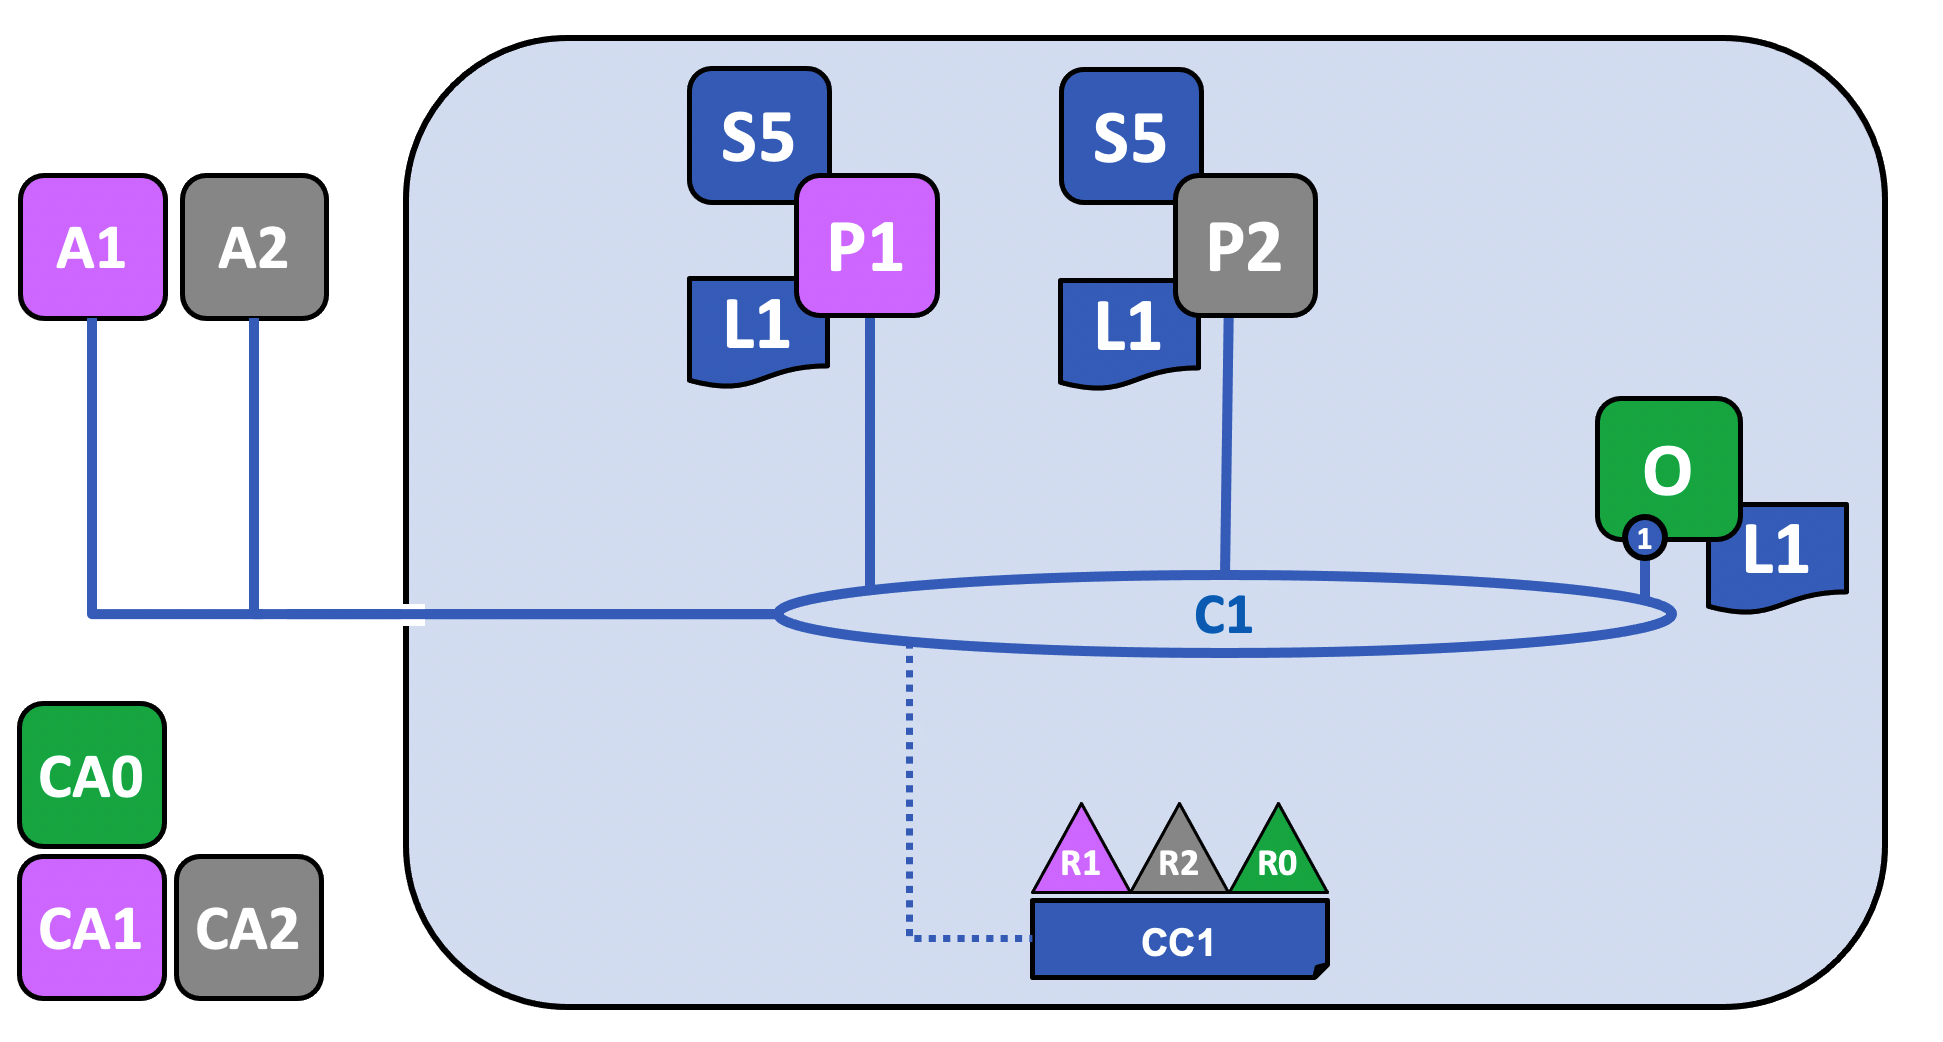
\includegraphics[width=0.9\textwidth]{images/network.png}
    \caption{Mạng Blockchain Hyperledger Fabric }
    \label{fig:network}
\end{figure}

Các thành phần trong mạng là:
\begin{itemize}
    \item[-] \textbf{CC:} Channel Configuration (Cấu hình của kênh).
    \item[-] \textbf{R:} Organization (Tổ chức).
    \item[-] \textbf{C:} Channel (Kênh), tập hợp các tổ chức có vai trò nhất định 
    trong cùng một quy trình kinh doanh. Ví dụ, trong một channel về mua bán 
    xe hơi sẽ gồm có 2 tổ chức là : Nhà sản xuất xe hơi, Nhà phân phối xe hơi.  
    \item[-] \textbf{P:} Peer (Nút thành viên) là điểm tương tác giữa các thành viên 
    trong tổ chức tương ứng với kênh, mọi hành động của người dùng đều 
    phải đi qua nó.
    \item[-] \textbf{O:} Orderer Node (Nút đặt hàng) tạo thành dịch vụ đặt hàng của kênh.
    \item[-] \textbf{L:} Ledger (Sổ cái) lưu trữ toàn bộ lịch sử giao dịch của kênh.
    \item[-] \textbf{A:} Application, ứng dụng hay giao diện (web, mobile app ) giúp người dùng tương tác với hệ thống dễ dàng hơn.
    \item[-] \textbf{CA:} Certificate Authority, phát hành danh tính cho người dùng 
    hoặc nút của tổ chức tương ứng. Ví dụ, người dùng A1 là thành viên của 
    Tổ chức R1, khi muốn tham gia vào mạng thì sẽ gửi yêu cầu đến CA1, 
    sau đó CA1 sẽ tạo ra một danh tính gồm khóa bí mật, khóa công khai và các 
    đặc tính liên quan khác, sau đó trả về cho người dùng A1, từ đó về sau 
    A1 dùng danh tính đó để thực hiện các tương tác với mạng, mạng sẽ tự động 
    biết đó là người dùng A1 đến từ tổ chức R1.
    \item[-] \textbf{S:} Smart Contract (Chaincode) được cài đặt trên kênh, định nghĩa rõ các hành động mà có thể thực hiện trên kênh.
    
\end{itemize}

Các bước để tạo một mạng Fabric:

\subsubsection{Tạo cơ sở mạng}

\begin{figure}[h]
    \centering
    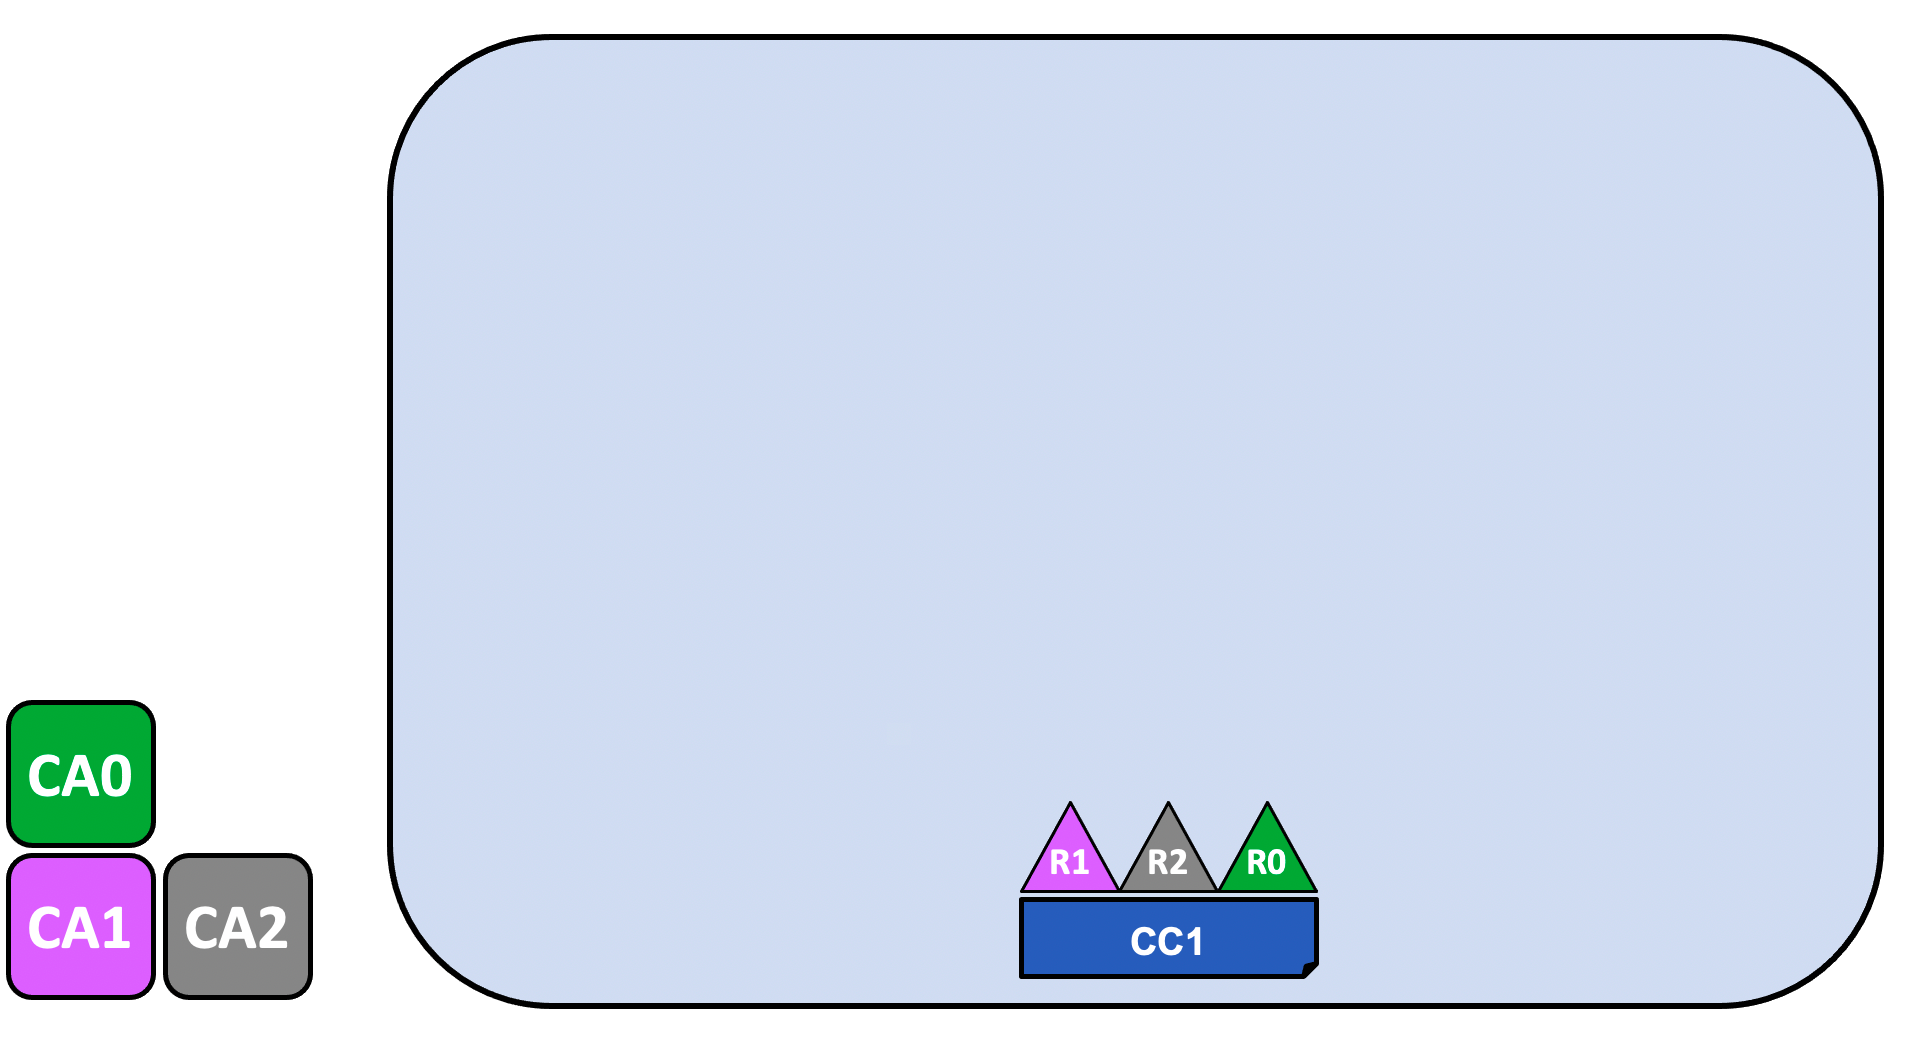
\includegraphics[width=0.8\textwidth]{images/create_network.png}
    \caption{Tạo mạng }
\end{figure}
Đầu tiên, các tổ chức R1, R2, R3 đồng ý sử dụng cấu hình CC1. Khối cấu hình được tạo. 
Khối cấu hình này chứa một bản ghi về các tổ chức có thể tham gia các thành phần và 
tương tác trên kênh, cũng như các chính sách xác định cấu trúc về cách đồng thuận để được các kết quả cụ thể.

Danh tính của các tổ chức này và danh tính của quản trị viên của họ phải 
được tạo bởi Tổ chức phát hành chứng chỉ (CA) được liên kết với từng tổ chức.

\subsubsection*{Tổ chức phát hành chứng chỉ (CA)}

Tổ chức phát hành chứng chỉ là một dịch vụ xác thực và quản lý chứng chỉ số trong hệ thống Hyperledger 
Fabric. Nó cung cấp các tính năng quản lý chứng chỉ số, chứng nhận, đăng ký và phân phối cho các thành 
phần trong mạng Hyperledger Fabric.

Các tính năng chính của CA bao gồm:

\begin{itemize}
    \item[-] Đăng ký danh tính cho các thành phần trong mạng: rootCert
    \item[-] Cấp giấy chứng nhận tuyển sinh (ECert): Khóa bí mật và công khai được tạo bởi ứng dụng khách Fabric CA, sau đó gửi khóa công khai
    đến CA để được trả về chứng chỉ.
    \item[-] Cấp, đổi, thu hồi chứng chỉ
\end{itemize}



Các thành phần khác nhau của blockchain sử dụng các chứng 
chỉ để xác định lẫn nhau là từ một tổ chức cụ thể. Ở ví dụ tạo mạng trên, 
ta có 3 CA đại điện cho 3 tổ chức.


CA tạo danh tính bằng cách tạo khóa công khai và khóa riêng tạo thành một cặp khóa có thể được sử dụng 
để chứng minh danh tính. Để xác định danh tính, ta phải cần một cơ quan đáng tin cậy đó là Nhà cung cấp dịch vụ thành viên (MSP).

MSP là một tập hợp các thư mục được thêm vào cấu hình mạng của kênh và được sử dụng để xác định 
quyền thực thi của tổ chức. MSP chứa danh sách danh tính được chấp nhận trong kênh, chức 
vụ và xác định quyền cho một nút trên kênh. 


\subsubsection{Các nút tham gia vào kênh}

\begin{figure}[h]
    \centering
    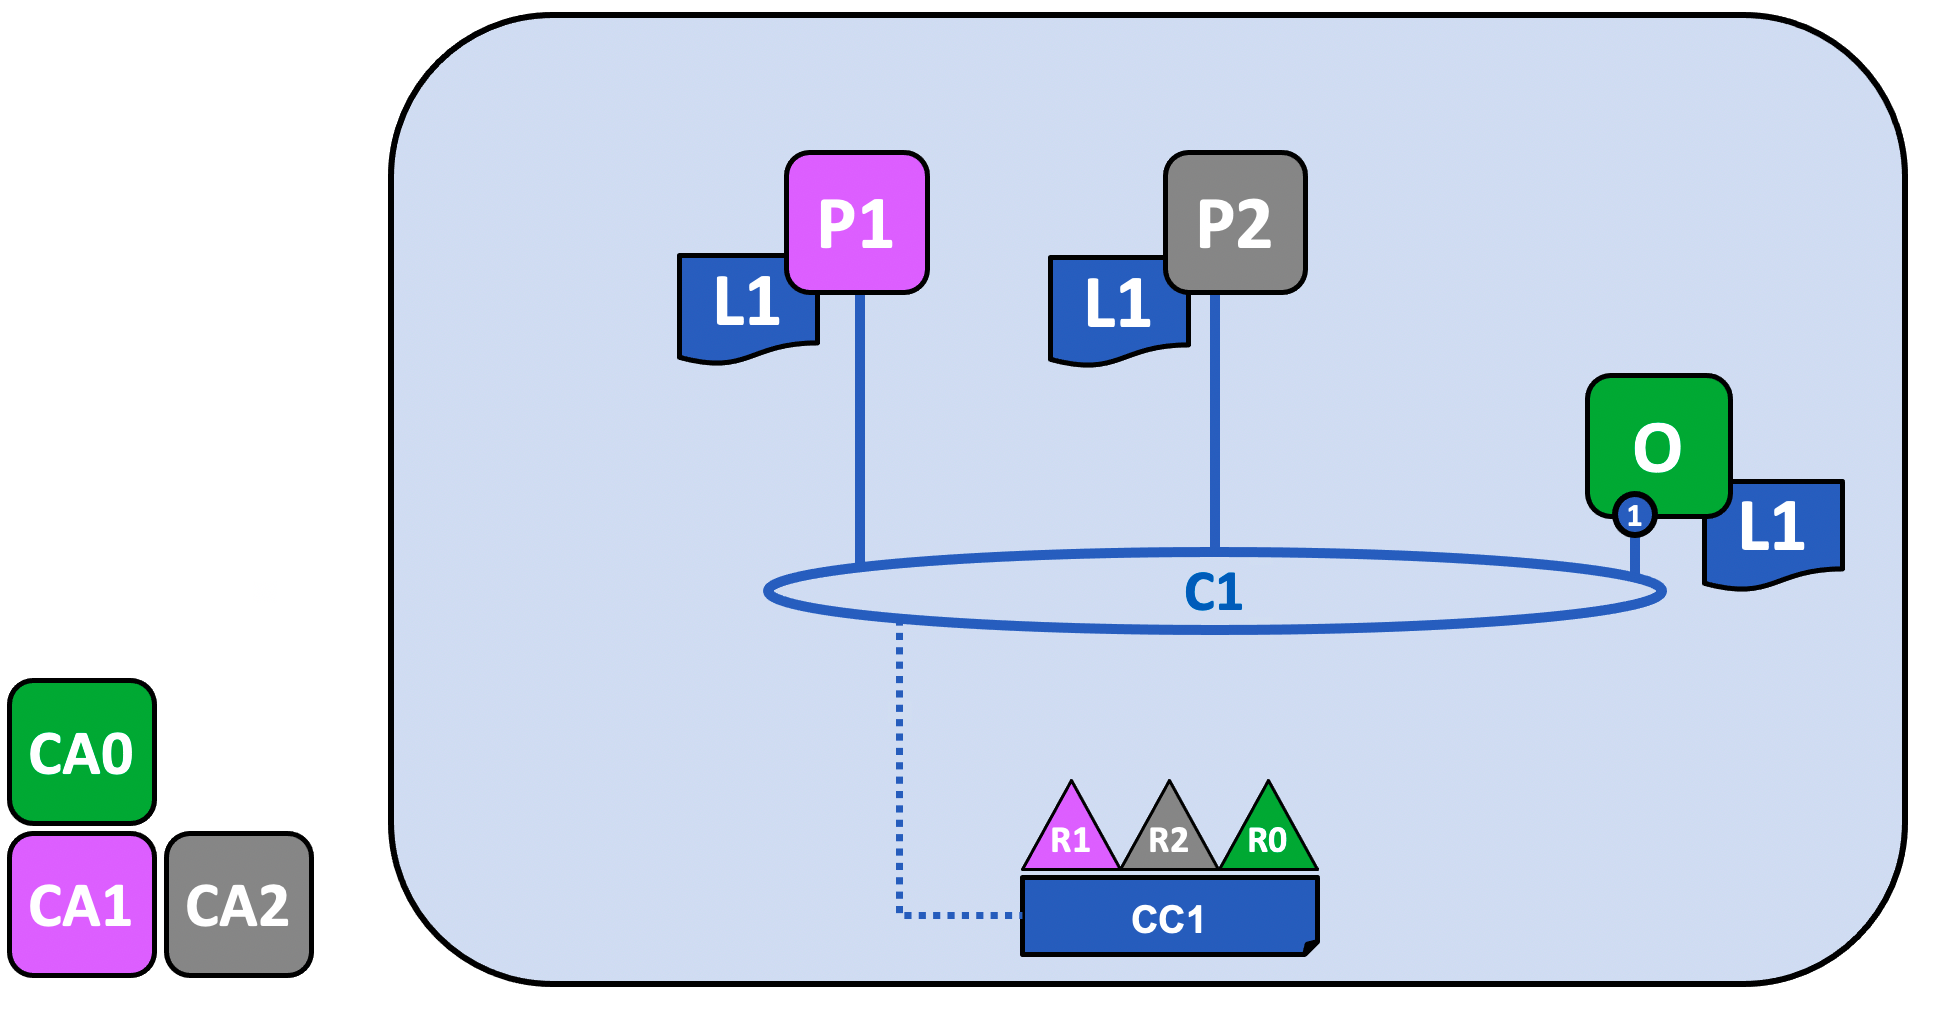
\includegraphics[width=0.9\textwidth]{images/join_network.png}
    \caption{Các nút tham gia vào kênh }
\end{figure}

Các nút thành viên, đặt hàng tham gia vào kênh. Các nút thuộc về mỗi tổ chức có chứng chỉ x.509 do Cơ quan cấp chứng chỉ 
liên kết với tổ chức đó tạo cho chúng. Chứng chỉ của P1 được tạo bởi CA1, chứng chỉ của P2 được tạo 
bởi CA2, v.v.

\subsubsection{Cài đặt và khởi tạo chaincode}

Chaincode được cài đặt trên các nút thành viên, sau đó được khởi tạo trên kênh. 

\begin{figure}[h]
    \centering
    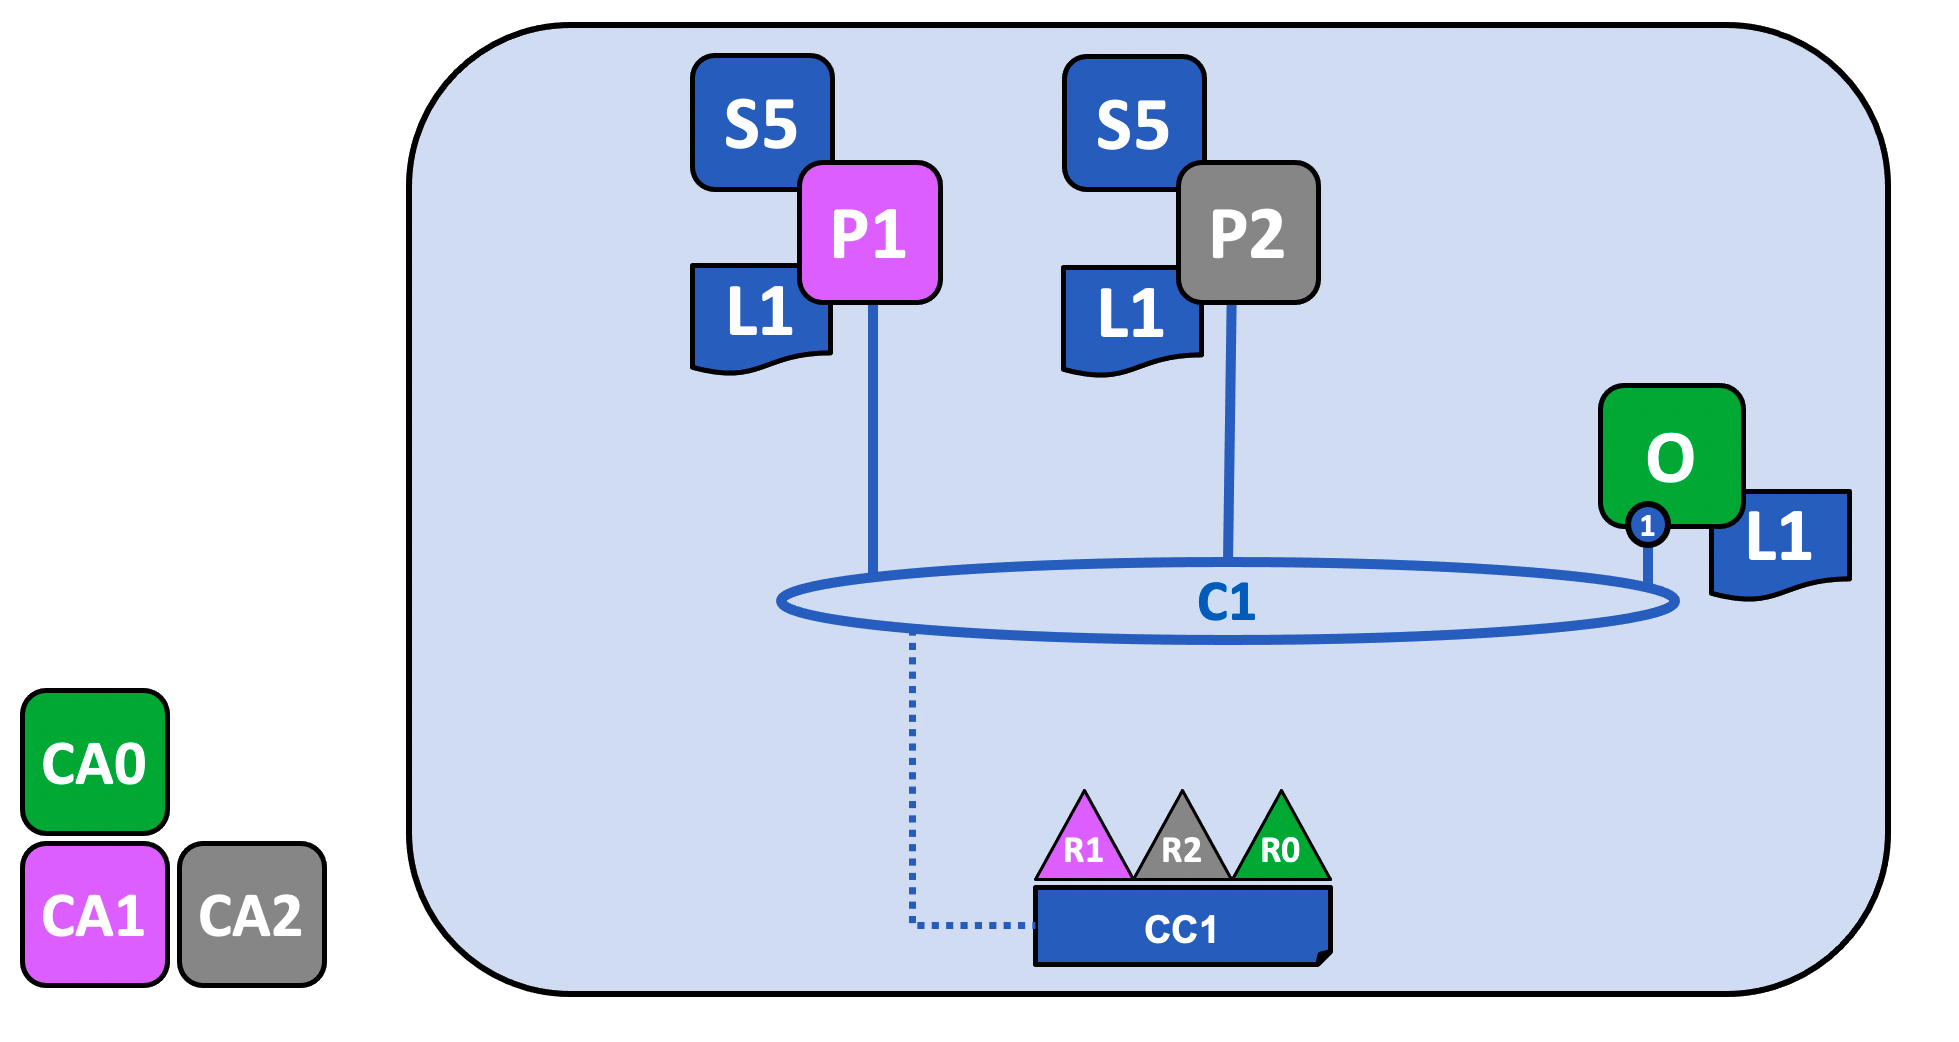
\includegraphics[width=0.9\textwidth]{images/install_chaincode.png}
    \caption{Cài đặt và khởi tạo chaincode}
\end{figure}

\subsubsection{Thêm ứng dụng khách trên kênh}

Sau khi hợp đồng thông minh đã được cam kết, các ứng dụng khách có thể được sử dụng để gọi 
các giao dịch thông qua các hàm chaincode. Sau bước này, mạng đã sẵn sàng để sử dụng.
Mạng được tạo sẽ có cấu trúc như hình \ref{fig:network}.

\subsection{Luồng giao dịch}
\label{subsec:luonggiaodich}
Luồng giao dịch có các bước sau:
\begin{figure}[h]
    \centering
    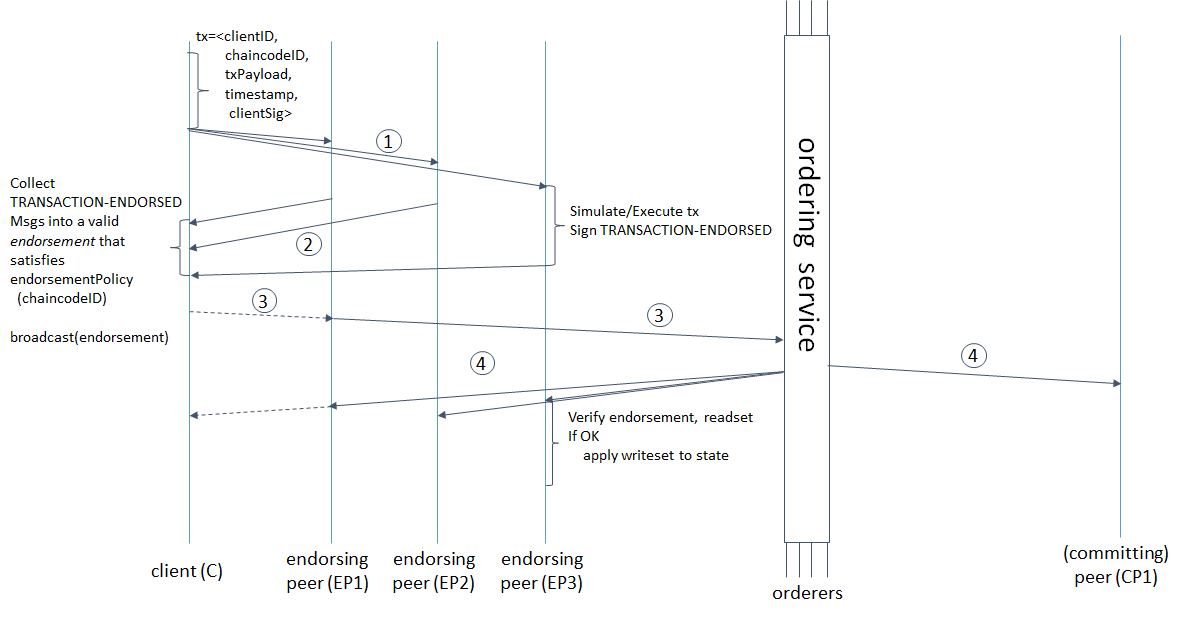
\includegraphics[width=1\textwidth]{images/flow-4.png}
    \caption{Luồng giao dịch }
\end{figure}


\begin{itemize}
    \item[\textbf{1.}] Khách gửi một giao dịch đến các  nút biểu quyết. Nút biểu quyết được sử dụng để chứng nhận tính hợp 
    lệ của một giao dịch trước khi nó được gửi đến các nút khác để xác nhận và cam kết trên 
    sổ cái. Nó không lưu trữ trực tiếp các thông tin liên quan đến giao dịch hoặc sổ cái.
    \item[\textbf{2.}] Khi một giao dịch được gửi đến nút biểu quyết, nó sẽ thực hiện một số hoạt 
    động để chứng nhận tính hợp lệ của giao dịch đó. Đầu tiên, nó sẽ kiểm 
    tra giao dịch này đã từng được gửi hay chưa để đảm bảo không trùng lặp. Chaincode sẽ được thực thi
    và trả về kết quả. Với mỗi một lệnh được thực hiện thì ta ghi lại 
    trạng thái đọc và ghi của dữ liệu, gọi là tập ReadWrite (RW).
    Nếu nút này thấy là giao dịch hợp lệ, nó sẽ tạo một chữ ký bảo lãnh. Tập RW cùng chữ ký sẽ được gửi lại cho người 
    gửi giao dịch. 
    \item[\textbf{3.}] Khi một giao dịch được ký chữ ký bảo lãnh, khách sẽ gửi giao dịch
    đó đến các ordering service. Người đặt hàng sẽ xác định thứ tự của các khối dựa trên 
    chữ ký bảo lãnh của nút biểu quyết và sắp xếp các giao dịch vào các khối tương 
    ứng. Sau đó nó gửi các khối đến toàn bộ nút thành viên.
    \item[\textbf{4.}] Người xác thực kiểm tra lại chính sách xác thực và kiểm tra hiệu lực của tập RW. Việc xác nhận giao dịch sẽ được lưu vào World- state, còn sổ cái sẽ lưu lại các giao dịch. 
    Khối sẽ được đánh dấu là hợp lệ hoặc không hợp lệ.
    \item[\textbf{5.}] Nếu khối là hợp lệ. Khối sẽ được thêm vào chuỗi. Các nút thành viên cập nhật lại trạng thái của sổ cái theo giao thức đồng thuận Raft.
    Thông báo lại kết quả cho ứng dụng khách. \cite{hyperledger}
\end{itemize}

\chapter{ Truy xuất nguồn gốc thực phẩm dựa trên công nghệ Blockchain}
\section{Đặt vấn đề}

Như đã trình bày ở chương \ref{Chapter2}, ta cần tìm ra một mô hình có thể đảm bảo 
tính toàn vẹn và đáng tin cậy cao, khó bị tấn công từ bên ngoài, và giúp 
cải thiện tính minh bạch và đáng tin cậy trong quá trình sản xuất và vận 
chuyển sản phẩm.  

Bài toán truy xuất nguồn gốc thực phẩm là một trong những ứng dụng tiềm năng của công nghệ 
blockchain. Bằng cách sử dụng blockchain, thông tin về nguồn gốc, vận chuyển và lưu trữ 
của các sản phẩm thực phẩm có thể được lưu trữ và truy xuất một cách an toàn và minh bạch.
\subsection{Ưu điểm mô hình truy xuất nguồn gốc thực phẩm dựa trên blockchain}
 
\begin{itemize}
    \item \textbf{Minh bạch:} Các thông tin về nguồn gốc, vận chuyển và lưu trữ của các sản phẩm 
    thực phẩm được lưu trữ và truy xuất một cách an toàn và minh bạch.
    \item \textbf{An toàn:} Các thông tin về nguồn gốc, vận chuyển và lưu trữ của các sản phẩm 
    thực phẩm được lưu trữ và truy xuất một cách an toàn và minh bạch.
    \item \textbf{Đáng tin cậy:} Các thông tin về nguồn gốc, vận chuyển và lưu trữ của các sản phẩm 
    thực phẩm được lưu trữ và truy xuất một cách an toàn và minh bạch.
\end{itemize}

\subsection{Cách tiếp cận và giải pháp}

Sử dụng nền tảng Hyperledger Fabric để xây dựng một mạng lưới blockchain phù hợp với 
mục đích truy xuất nguồn gốc thực phẩm.

\section{Mô hình hệ thống}
\subsection{Các thành phần tham gia}

Cốt lõi của hệ thống được thực hiện dưới dạng chaincode. Chaincode cung cấp các thao tác cho phép người dùng hệ thống thêm và sửa đổi 
thông tin trong blockchain một cách an toàn và có thể theo dõi được. Người sử dụng hệ thống
là các thành viên chuỗi cung ứng và các bộ phận quản lý. Các thực thể tham gia 
vào hoạt động của hệ thống là các tổ chức người dùng, trong đó mỗi người dùng được xác định 
bằng một chứng chỉ do cơ quan chứng nhận liên kết với tổ chức được xác định rõ ràng mới có thể 
tham gia vào các hoạt động của hệ thống. Trong Hyperledger Fabric, tập hợp các tổ chức tham 
gia vào các hoạt động blockchain được xác định trước. Hyperledger Fabric cho phép thêm một tổ 
chức mới hoặc xóa một tổ chức hiện có trong thời gian chạy bằng cách chuyển một loạt các 
giao dịch sang blockchain phải được đa số các tổ chức tham gia chấp thuận.

Với hệ thống truy xuất nguồn gốc thực phẩm, thành viên bao gồm: 
\begin{itemize}
    \item[-] Nhà cung cấp giống vật tư: Dữ liệu truy tìm bao gồm thông tin về nguyên liệu 
    thực phẩm nông nghiệp (ví dụ: hạt giống, thuốc trừ sâu và phân bón), giao dịch với người nông dân v.v.
    \item[-] Nông dân: Dữ liệu truy tìm bao gồm thông tin về các trang trại, quá trình canh tác,
    điều kiện thời tiết, giao dịch với các nhà sản xuất, ...
    \item[-] Nhà sản xuất: Dữ liệu truy tìm bao gồm thông tin về các nhà máy, quá trình sản xuất,
    giao dịch với nông dân và nhà phân phối,...
    \item[-] Công ty vận chuyển: Dữ liệu truy tìm bao gồm chi tiết vận chuyển, điều kiện lưu trữ, giao
    dịch với nông dân, nhà phân phối hay nhà sản xuất,...
    \item[-] Nhà phân phối: Dữ liệu truy tìm bao gồm thông tin về các cửa hàng, quá trình phân phối,
    ngày nhập hàng, hạn sử dụng, các giao dịch với nhà sản xuất,...
\end{itemize}

Tuỳ vào từng sản phẩm cụ thể, mô hình có thể thêm hoặc bớt các thành viên tham gia. 
\subsection{Phân tích và thiết kế hệ thống}
\subsubsection{Domain Model}

\begin{figure}[h]
    \centering
    \includegraphics[width=0.7\textwidth]{images/domain_model.png}
    \caption{Domain Model của Business Logic \cite{app}} 
\end{figure}

Các tổ chức muốn tham gia vào chuỗi cung ứng sẽ đăng ký tham gia. Để được xác nhận, 
tổ chức sẽ kí hợp đồng thông minh thể hiện qua chaincode. Nếu thoả mãn hợp đồng, 
tổ chức sẽ được thêm vào và có một mã định danh ID. Chaincode thể hiện các điều khoản
và các cam kết cần thực hiện. 

Một loại sản phẩm muốn thêm vào blockchain sẽ được đăng ký thông qua một hợp đồng 
thông minh. Nó thoả mãn các yêu cầu thì sẽ được thêm vào blockchain. Việc kiểm tra 
yêu cầu này được thực hiện một cách tự động thông qua các hàm của chaincode. Sản phẩm có một 
số thuộc tính như ID, type, state,...
Một sản phẩm có thể được cấu tạo từ nhiều nguyên liệu, vật tư,... Những nguyên liệu ấy
có thể đã được tồn tại trong mạng blockchain. Nếu tồn tại trong mạng blockchain, ta sẽ thêm 
thuộc tính params để thể hiện mối quan hệ. Nếu không thì ta sẽ yêu cầu giao dịch
để ghi thông tin về sản phẩm. 

Việc xây dựng Domain Model như này giúp việc quản lý nguồn gốc cũng như xác thực nguồn gốc 
dễ dàng hơn, như quản lý được sản phẩm được sản xuất từlô nông sản nào, cũng từ đó truy xuất được nguồn gốc giống của sản phẩm nôngsản.
\subsubsection{Chaincode (Hợp đồng thông minh)}
Chaincode nó được sử dụng để xác định các đầu vào và đầu ra của các giao dịch trên blockchain. Chaincode là một chương trình được 
viết bằng một trong các ngôn ngữ lập trình.

Một số hàm tiêu biểu của chaincode trong hệ thống truy xuất nguồn gốc thực phẩm.

\begin{itemize}
    \begin{figure}[h]
        \centering
        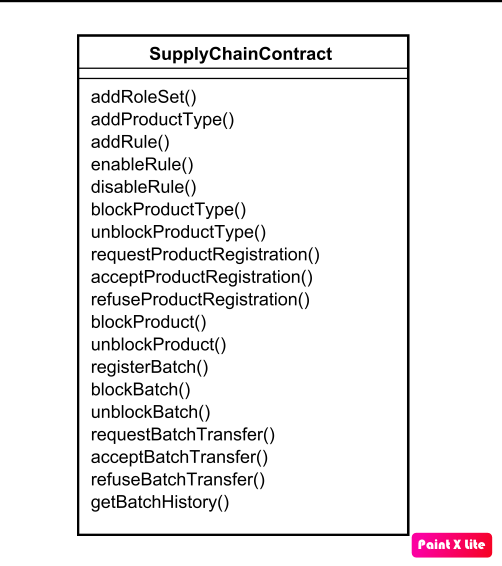
\includegraphics[width=0.4\textwidth]{images/Smart_Contract.png}
        \caption{Chaincode \cite{app}}
    \end{figure}
    \item \textbf{addRoleSet():} Thêm một thành viên mới vào hệ thống. Thành viên này có thể là một tổ chức hoặc cá nhân.
    \item \textbf{addProductType():} Thêm một loại sản phẩm mới vào hệ thống. Loại sản phẩm này có thể là sản phẩm chính hoặc sản phẩm phụ.
    \item \textbf{addRule():} Thêm một quy tắc mới vào hệ thống. Quy tắc này có thể là quy tắc chính hoặc quy tắc phụ.
    \item \textbf{enableRule () và disableRule ():} Cho phép bật và tắt rule qua ruleId.
    \item \textbf{blockProductType() và unblockProductType():} cho phép chặn và mở chặn một loại sản phẩm.
    \item \textbf{requestProductRegistration():} yêu cầu đăng ký một sản phẩm mới.
    \item \textbf{acceptProductRegistration() và refuseProductRegistration():} cho phép chất nhận hoặc từ chối đăng ký sản phẩm.
    \item \textbf{blockProduct() và unblockProduct():} cho phép chặn và mở chặn một sản phẩm.
    \item \textbf{registerBatxh():} cho phép một tổ chức đăng ký một lô sản phẩm liên kết với sản phẩm nào đó.
    \item \textbf{blockBatch() và unblockBatch():} cho phép chặn và mở chặn một lô sản phẩm.
    \item \textbf{requestBatchTransfer():} cho phép một tổ chức yêu cầu chuyển một lô sản phẩm từ một tổ chức khác.
    \item \textbf{acceptBatchTransfer() và refuseBatchTransfer():} cho phép chấp nhận hoặc từ chối chuyển lô sản phẩm.
    \item \textbf{getBatchHistory():} cho phép lấy lịch sử của một lô sản phẩm.
\end{itemize}
\subsubsection{Tạo mạng}
\subsection{Các bước thực hiện}
Các bước thực hiện cơ bản của hệ thống truy xuất nguồn gốc thực phẩm như sau:
\begin{itemize}
    \item[-] \textbf{Bước 1:} Các tổ chức đăng ký thành viên vào hệ thống.
        \item[-] \textbf{1.1:} Các tổ chức tạo nút thành viên. 
        \item[-] \textbf{1.2:} Các nút thành viên tham gia vào kênh.
        \item[-] \textbf{1.3:} Tổ chức tạo admin là nút khách trong hệ thống, và yêu cầu
        tham gia vào kênh. Peer node xác thực thông tin của client và cấp quyền.
    \item[-] \textbf{Bước 2:} Các tổ chức đăng ký các loại sản phẩm của riêng mình bằng cách 
    gửi yêu cầu giao dịch. Các bước thực hiện được trình bày ở \ref{subsec:luonggiaodich} của chương \ref{chap:hyper}.
    \item[-] \textbf{Bước 3:} Các tổ chức lần lượt thêm các thông tin, các thông tin sẽ được
    lưu trữ trong các khối nối tiếp nhau và sắp xếp theo thời gian. Các nút thành viên sẽ lưu 
    trữ chuỗi khối này ở sổ cái.
    \item[-] \textbf{Bước 4:} Khách hàng đăng nhập vào ứng dụng và nhập mã để yêu cầu truy xuất
    thông tin sản phẩm. Nếu sản phẩm chỉ thuộc 1 kênh, không có nguyên liệu thuộc kênh
    khác thì sẽ trả về thông tin sản phẩm. Ngược lại thì sẽ truy xuất thông tin nguyên liệu
    của sản phẩm đó và trả về tất cả thông tin sản phẩm.
\end{itemize}


\section{Công nghệ sử dụng}
- Docker

- Golang

- Hyperledger Fabric

\section{Thực nghiệm}

\section{Kết luận và hướng phát triển}

\begin{thebibliography}{1}
    \subsection*{Tiếng Anh}
    \setlength{\bibindent}{1cm}
    \setlength{\itemindent}{-\bibindent}
  
    \bibitem{Sha256}
      What is SHA-256? (2020).
      Retrieved from

    \url{https://blog.boot.dev/cryptography/how-sha-2-works
    -step-by-step-sha-256/}.
  
        
    \bibitem{Diffie_Hellman}
    \raggedright
    Jeffrey Hoffstein, Jill Pipher and Joseph H. Silverman (2014),
    ``Discrete Logarithms and Diffie-Hellman'',
    \emph{An Introduction to Mathematical Cryptography},
    pp. 65-67.

    \bibitem{Elliptic_Curve}
    \raggedright
    Jeffrey Hoffstein, Jill Pipher and Joseph H. Silverman (2014),
    ``Elliptic Curves and Cryptography'',
    \emph{An Introduction to Mathematical Cryptography},
    pp. 279-299.
    \bibitem{ECDSA}
    \raggedright
    Jeffrey Hoffstein, Jill Pipher and Joseph H. Silverman (2014),
    ``Digital Signatures'',
    \emph{An Introduction to Mathematical Cryptography},
    pp. 442-447.
  \end{thebibliography}

\listoffigures
\newpage
\chapter*{Danh mục các cụm từ dịch sang tiếng Anh}
\addcontentsline{toc}{chapter}{Danh mục các cụm từ dịch sang tiếng Anh}

\begin{table}[htbp]
  \fontsize{14}{18}\selectfont
    \begin{center}
      \begin{tabular*}{\linewidth}{@{\extracolsep{\fill}}|>{\centering}m{0.1\linewidth}|>{\centering\arraybackslash}m{0.4\linewidth}|>{\centering\arraybackslash}m{0.4\linewidth}|}
        \hline
        \textbf{STT} & \textbf{Tiếng Việt} &  \textbf{Tiếng Anh} \\
        \hline
        01 & Hàm băm & Hash Function  \\
        \hline
        02 & Bản rõ &  Plaintext \\
        \hline
        03 & Bản mã &  Ciphertext \\
        \hline
          04 & Khoá công khai &  Pubblic Key \\
        \hline
          05 & Khoá bí mật &  Private Key \\
        \hline
        06 & Giá trị băm & Hash Value \\
        \hline
        07 & Cây Merkle & Merkle Tree\\
        \hline
        08 & Khối & Block \\
        \hline
        09 & Chuỗi khối & Blockchain \\
        \hline
        10 & Nút & Node \\
        \hline
        11 & Giao thức đồng thuận & Consensus Protocol\\
        \hline
        12 & Cấu trúc phi tập trung & Decentralized Structure \\
        \hline
        13 & Mạng ngang hàng & Peer-to-peer Network \\
        \hline
        14 & Bằng chứng công việc & Proof of Work \\
        \hline
        15 & Bằng chứng cổ phần & Proof of Stake \\
        \hline
        16 & Hợp đồng thông minh & Smart Contract \\
        \hline
        17 & Chữ ký bảo lãnh & Endorsement Signature \\
        \hline
        18 & Nút biểu quyết & Endorsing Peer \\
        \hline
        19 & Nút xác thực & Proposing Peer \\
        \hline
      \end{tabular*}
    \end{center}
  \end{table}
  




\end{document}      